\documentclass[10pt]{beamer}

\usetheme{metropolis}
\usepackage{appendixnumberbeamer}

\usepackage[]{algorithm2e}
% \usepackage{algorithm}
% \usepackage{algpseudocode}
\usepackage{amsfonts}
\usepackage[ngerman]{babel}
\usepackage[backend=biber]{biblatex}
\usepackage{booktabs}
\usepackage[scale=2]{ccicons}
\usepackage{graphicx}
\usepackage{hyperref}
\usepackage[utf8]{inputenc} 
\usepackage{lipsum}
\usepackage{listings}
\usepackage{multirow}

\usepackage{pgfplots}
\usepackage{xcolor}

\addbibresource{presentation.bib}

\SetInd{0.25em}{0.4em}

\usepgfplotslibrary{dateplot}

\usepackage{xspace}

\setbeamertemplate{frametitle continuation}{}

\newcommand{\themename}{\textbf{\textsc{metropolis}}\xspace}

\newcommand{\backupbegin}{
   \newcounter{framenumberappendix}
   \setcounter{framenumberappendix}{\value{framenumber}}
}

\newcommand{\backupend}{
   \addtocounter{framenumberappendix}{-\value{framenumber}}
   \addtocounter{framenumber}{\value{framenumberappendix}} 
}

\addto{\captionsngerman}{%
  \renewcommand*{\figurename}{Abb.}
}

\let\svthefootnote\thefootnote

\definecolor{mGreen}{rgb}{0,0.6,0}
\definecolor{mGray}{rgb}{0.5,0.5,0.5}
\definecolor{mPurple}{rgb}{0.58,0,0.82}

\lstdefinestyle{CStyle}{
    commentstyle=\color{mGreen},
    keywordstyle=\color{magenta},
    numberstyle=\tiny\color{mGray},
    stringstyle=\color{mPurple},
    basicstyle=\footnotesize,
    breakatwhitespace=false,
    breaklines=true,
    captionpos=b,
    keepspaces=true,
    numbers=left,
    numbersep=5pt,
    showspaces=false,
    showstringspaces=false,
    showtabs=false,
    tabsize=2,
    language=C
}

\title{Ein skalierbarer L\"oser f\"ur Randwertprobleme unter Verwendung der
       Greenschen Kreuzapproximationsmethode und GPUs}
\date{24. Oktober 2017}
\author{Bennet Carstensen}
\institute{Christian-Albrechts-Universität zu Kiel\\
           Institut für Informatik\\
           Scientific Computing}
% \titlegraphic{\hfill\includegraphics[height=1.5cm]{logo.pdf}}

\begin{document}

\maketitle

\begin{frame}{Agenda}
  \setbeamertemplate{section in toc}[sections numbered]
  \tableofcontents[hideallsubsections]
\end{frame}

\section{Einleitung}

\begin{frame}{Randwertprobleme}
  \begin{columns}
    \column{0.675\linewidth}
      \begin{itemize}
        \visible<1->{\item Wird verwendet in der Physik/Ingenieurwissenschaft
                     \begin{itemize}
                       \item Elektrostatik
                       \item Wärmeleitung
                       \item Akustik
                     \end{itemize}}
        \item \visible<1->{Sei \(\Omega \subseteq \mathbb{R}^{d}\) gegeben,
                           \( d \in \{ 2, 3 \} \)}
        \item \visible<2->{\( \int\limits_{\Omega} g(x, y) u(y) dy = f(x)
                              \newline \text{ für alle } x \in \Omega \)}
        \item \visible<2->{z.\,B. \(g(x, y) = \frac{1}{4\pi\left\lVert x - y
                           \right\rVert_{2}}\) (Fundamentallösung der
                           Laplace-Gleichung)}
      \end{itemize}
    \column{0.325\linewidth}
      \centering
      \begin{overprint}
        \onslide<1>\includegraphics[width=1.5\linewidth]{figures/fg-sphere-full.pdf}
        \onslide<2>\includegraphics[width=1.5\linewidth]{figures/fg-sphere-full-inf.pdf}
      \end{overprint}

  \end{columns}
  \footnotesize
  \let\thefootnote\relax\footnote{Steffen Börm und Sven Christophersen.
  \href{https://link.springer.com/article/10.1007\%2Fs00211-015-0757-y}{
  ``Approximation of integral operators by Green quadrature and nested cross 
  approximation''}. In: \textit{Numerische Mathematik} 133.3 (2016), S. 
  409-442, 2016.}
  \addtocounter{footnote}{-1}\let\thefootnote\svthefootnote\relax
  \normalsize
\end{frame}

\begin{frame}{Diskretisierung}
  \begin{columns}
    \column{0.675\linewidth}
      Galerkin-Diskretisierung mit Basisfunktionen\\
      \({(\varphi_{i})}_{i = 1}^{n} \text{ und }
        {(\psi_{j})}_{j = 1}^{n}, n \in \mathbb{N}\)
      \begin{itemize}
        \item \( V_{n} = \text{span}\{ \varphi_{i} : i \in \{ 1, \hdots, n\} \}
                \newline
                U_{n} = \text{span}\{ \psi_{j} : j \in \{ 1, \hdots, n\} \} \)
        \item Finde \(z = (z_{1}, \hdots, z_{n}) \in \mathbb{R}^{n} \) mit
              \( \sum\limits_{j = 1}^{n} \psi_{j} z_{j} \in U_{n} \) 
              und \( Gz = b \)
        \begin{itemize}
          \item \( g_{ij} = \int\limits_{\Omega} \varphi_{i}(x)
                   \int\limits_{\Omega} g(x, y) \ \psi_{j}(y) \ dy \ dx \)
          \item \(b_{i} = \int\limits_{\Omega} \varphi_{i}(x) \ f(x) \ dx\)
          \item \( i, j \in \{ 1, \hdots, n \} \)
        \end{itemize}
      \end{itemize}
    \column{0.325\linewidth}
      \centering
      \includegraphics[width=1.5\linewidth]{figures/fg-sphere-tri.pdf}
  \end{columns}
  \footnotesize
  \let\thefootnote\relax\footnote{Steffen Börm und Sven Christophersen.
  \href{https://link.springer.com/article/10.1007\%2Fs00211-015-0757-y}{
  ``Approximation of integral operators by Green quadrature and nested cross 
  approximation''}. In: \textit{Numerische Mathematik} 133.3 (2016), S. 
  409-442, 2016.}
  \addtocounter{footnote}{-1}\let\thefootnote\svthefootnote\relax
  \normalsize
\end{frame}

\begin{frame}{Probleme \& Lösungsansätze}
  \begin{overprint}
    \onslide<1-2>
      \begin{table}[h]
        \begin{tabular}{rrr} \toprule
          \multirow{2}{*}{Dimension} & \multicolumn{2}{c}{Speicherbedarf (in 
          GB)} \\ \cmidrule{2-3}
                      & Galerkin & \\ \midrule
              16\,384 &      1,0 & \\
              32\,768 &      4,0 & \\
              65\,536 &     16,0 & \\
             131\,072 &     64,0 & \\
             262\,144 &    256,0 & \\ \bottomrule
        \end{tabular}
      \end{table}
    \onslide<3>
      \begin{table}[h]
        \begin{tabular}{rrr} \toprule
          \multirow{2}{*}{Dimension} & \multicolumn{2}{c}{Speicherbedarf (in 
          GB)} \\ \cmidrule{2-3}
                      & Galerkin & \(\mathcal{H}^2\)-Matrix \\ \midrule
              16\,384 &      1,0 & 0,2 \\
              32\,768 &      4,0 & 0,4 \\
              65\,536 &     16,0 & 0,8 \\
             131\,072 &     64,0 & 1,8 \\
             262\,144 &    256,0 & 3,5 \\ \bottomrule
        \end{tabular}
      \end{table}
  \end{overprint}

  \begin{itemize}
    \item \visible<1->{Problem: \(G\) meist vollbesetzt \(\Rightarrow\) hohe
                       Speicheranforderungen und hoher Rechenaufwand}
    \visible<2->{\item Lösungsansätze:}
    \begin{itemize}
      \item \visible<2->{Schnelle Multipol-Methode (bessere
                         Laufzeitkomplexität)}
      \item \visible<3->{\(\mathcal{H}^2\)-Matrizen +
                           Greensche Kreuzapproximationsmethode\\
                           (engl. \textit{Green cross approximation [GCA]
                           method})\\
                           (geringere Speicheranforderungen \(\Rightarrow\)
                           bessere Laufzeitkomplexität)}
    \end{itemize}
  \end{itemize}
\end{frame}

\begin{frame}{Probleme \& Lösungsansätze}
  \begin{figure}
    \includegraphics[width=\linewidth]{figures/fg-memory-h2-nf-ff.pdf}
    \caption{Speicherbedarf einer \(\mathcal{H}^2\)-Matrix und derer 
             Blockmatrizen}
  \end{figure}
\end{frame}

\begin{frame}{Probleme \& Lösungsansätze}
  \begin{itemize}
    \item Problem: Reale Problemstellungen benötigen immer größere Matrizen
          \(\Rightarrow\) Selbst \(\mathcal{H}^2\)-Matrizen haben ihre Grenzen
    \item Lösungsansätze:
    \begin{itemize}
      \item Mehr Arbeitsspeicher
      \item Berechne reproduzierbare Untermatrizen einer
            \(\mathcal{H}^2\)-Matrix on-the-fly, wenn sie benötigt werden.
            (75--90\,\% des Speicherbedarfs wird eingespart.)
    \end{itemize}
  \end{itemize}
\end{frame}

\begin{frame}{Problem \& Lösungsansätze}
  \small
  \begin{table}[h]
    \begin{tabular}{rrr} \toprule
      \multirow{2}{*}{Dimension} & \multicolumn{2}{c}{Rechenzeit in
      ms\footnotemark[1]} \\ \cmidrule{2-3}
                & \(\mathcal{H}^2\)-MVM &
      \begin{tabular}{@{}c@{}}\(\mathcal{H}^2\)-MVM \\ on-the-fly\end{tabular} 
      \\ \midrule
        16\,384 &    140 &  6\,980 \\
        32\,768 &    300 & 14\,640 \\
        65\,536 &    660 & 29\,440 \\
       131\,072 & 1\,190 & 60\,920 \\ \bottomrule
    \end{tabular}
  \end{table}
  \normalsize
  \begin{itemize}
    \item Problem: Wesentlich größerer Rechenaufwand bei letzterem Ansatz
    \item Lösungsansatz (Thema dieser Master-Arbeit):
    \begin{itemize}
      \item Quadratur zur Auswertung der Integrale bestimmt Performance
      \item Quadratur ist äußerst parallelisierbar/vektorisierbar
      \item Auslagern der Auswertungen auf eine Grafikkarte
    \end{itemize}
  \end{itemize}
  \footnotesize
  \footnotetext[1]{Gleikommazahlen einfacher Genauigkeit auf einer Intel Xeon
                   E5-4640 mit OpenMP parallelisiert und AVX beschleunigt.}
  \normalsize
\end{frame}

\section{\(\mathcal{H}^2\)-Matrizen}

\begin{frame}{\(\mathcal{H}^2\)-Matrizen}
  Teile \( G \) rekursiv in Untermatrizen bzgl. \textit{zulässiger} und
  \textit{unzulässiger} Unteräume \( \tau \times \sigma \) auf

  \begin{columns}
    \column{.45\linewidth}
      \begin{figure}
        \begin{overprint}
          \onslide<1>\centering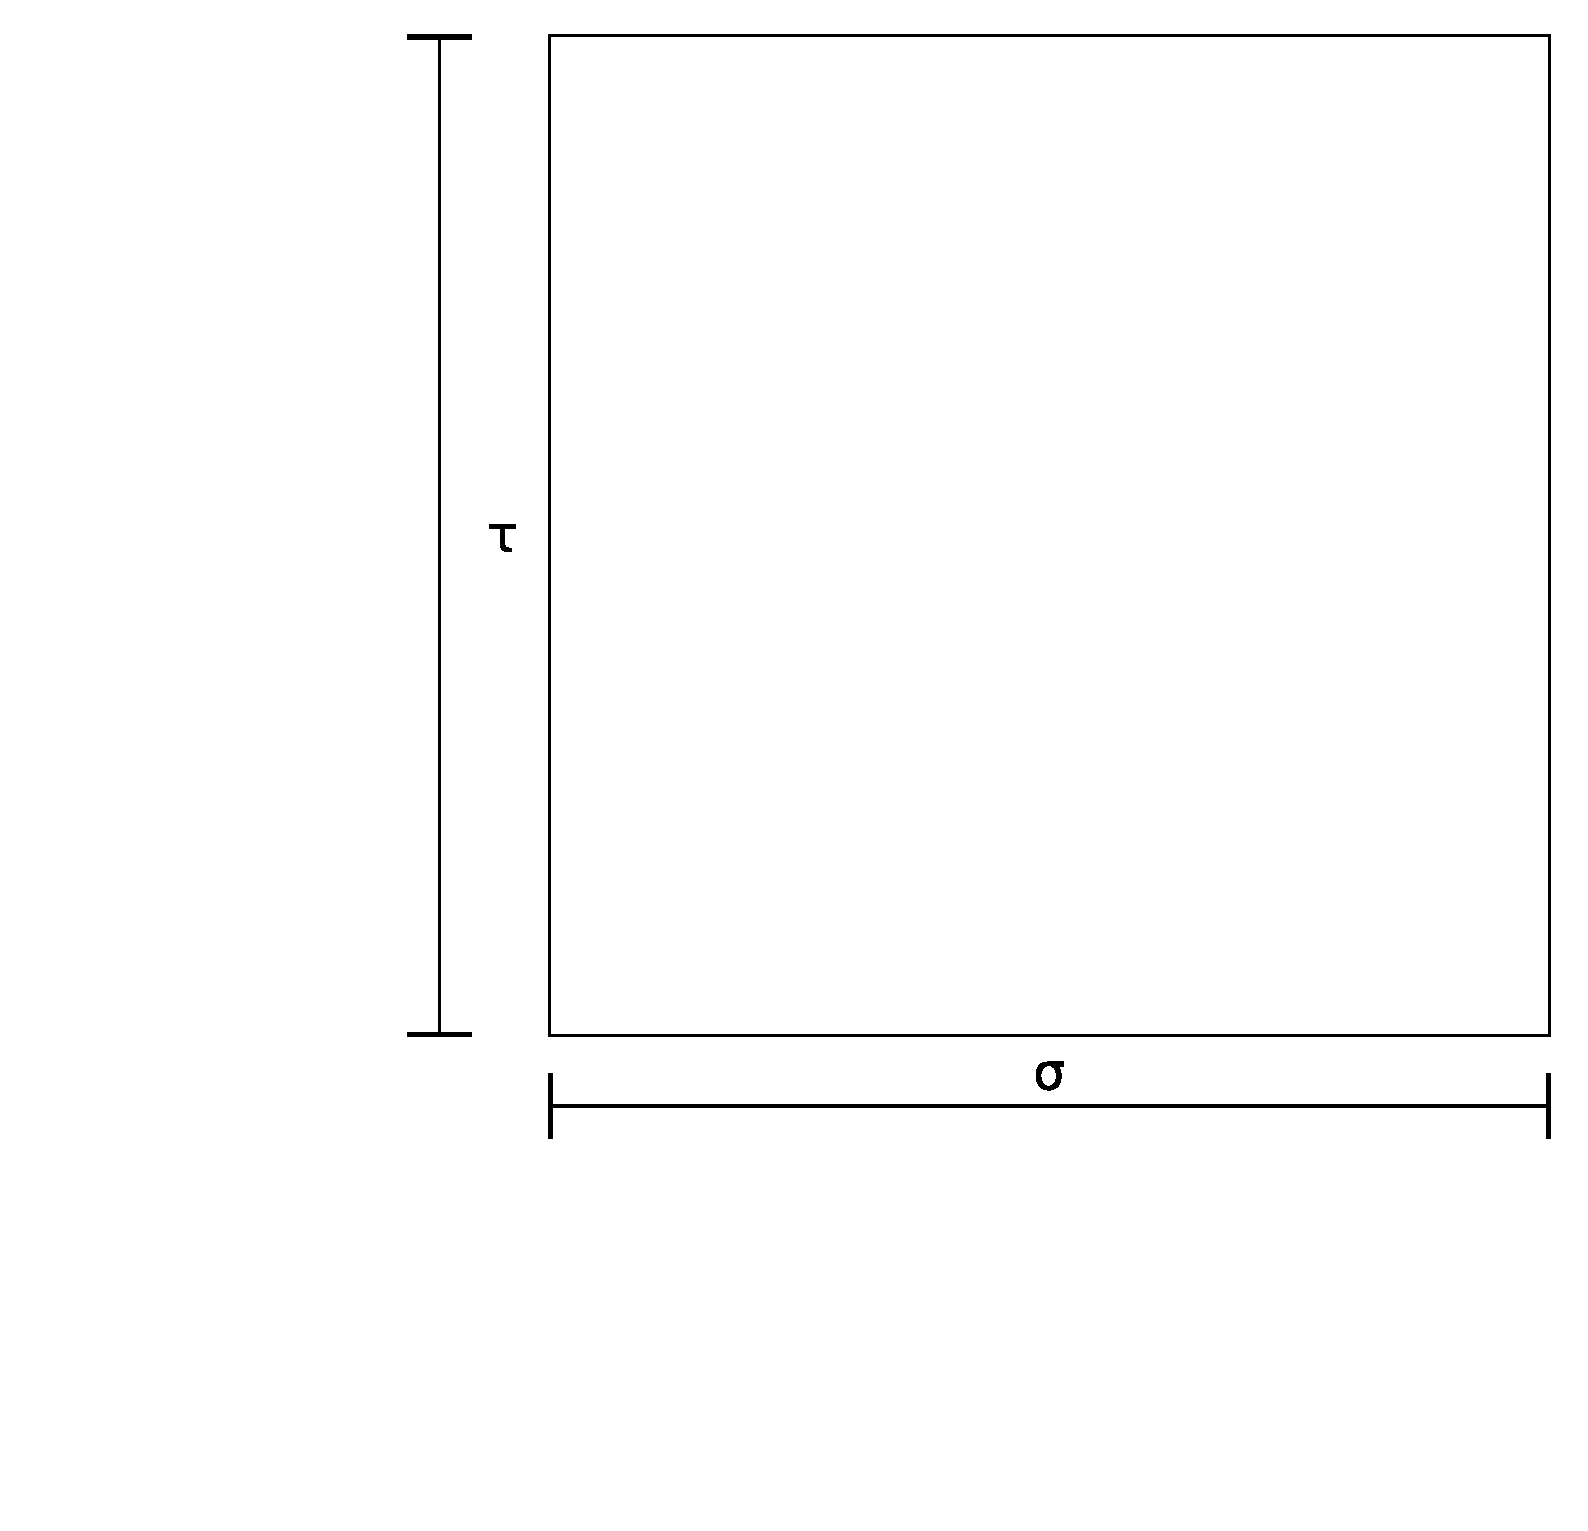
\includegraphics[width=\linewidth]{figures/fg-h2-matrix-1.pdf}
          \onslide<2>\centering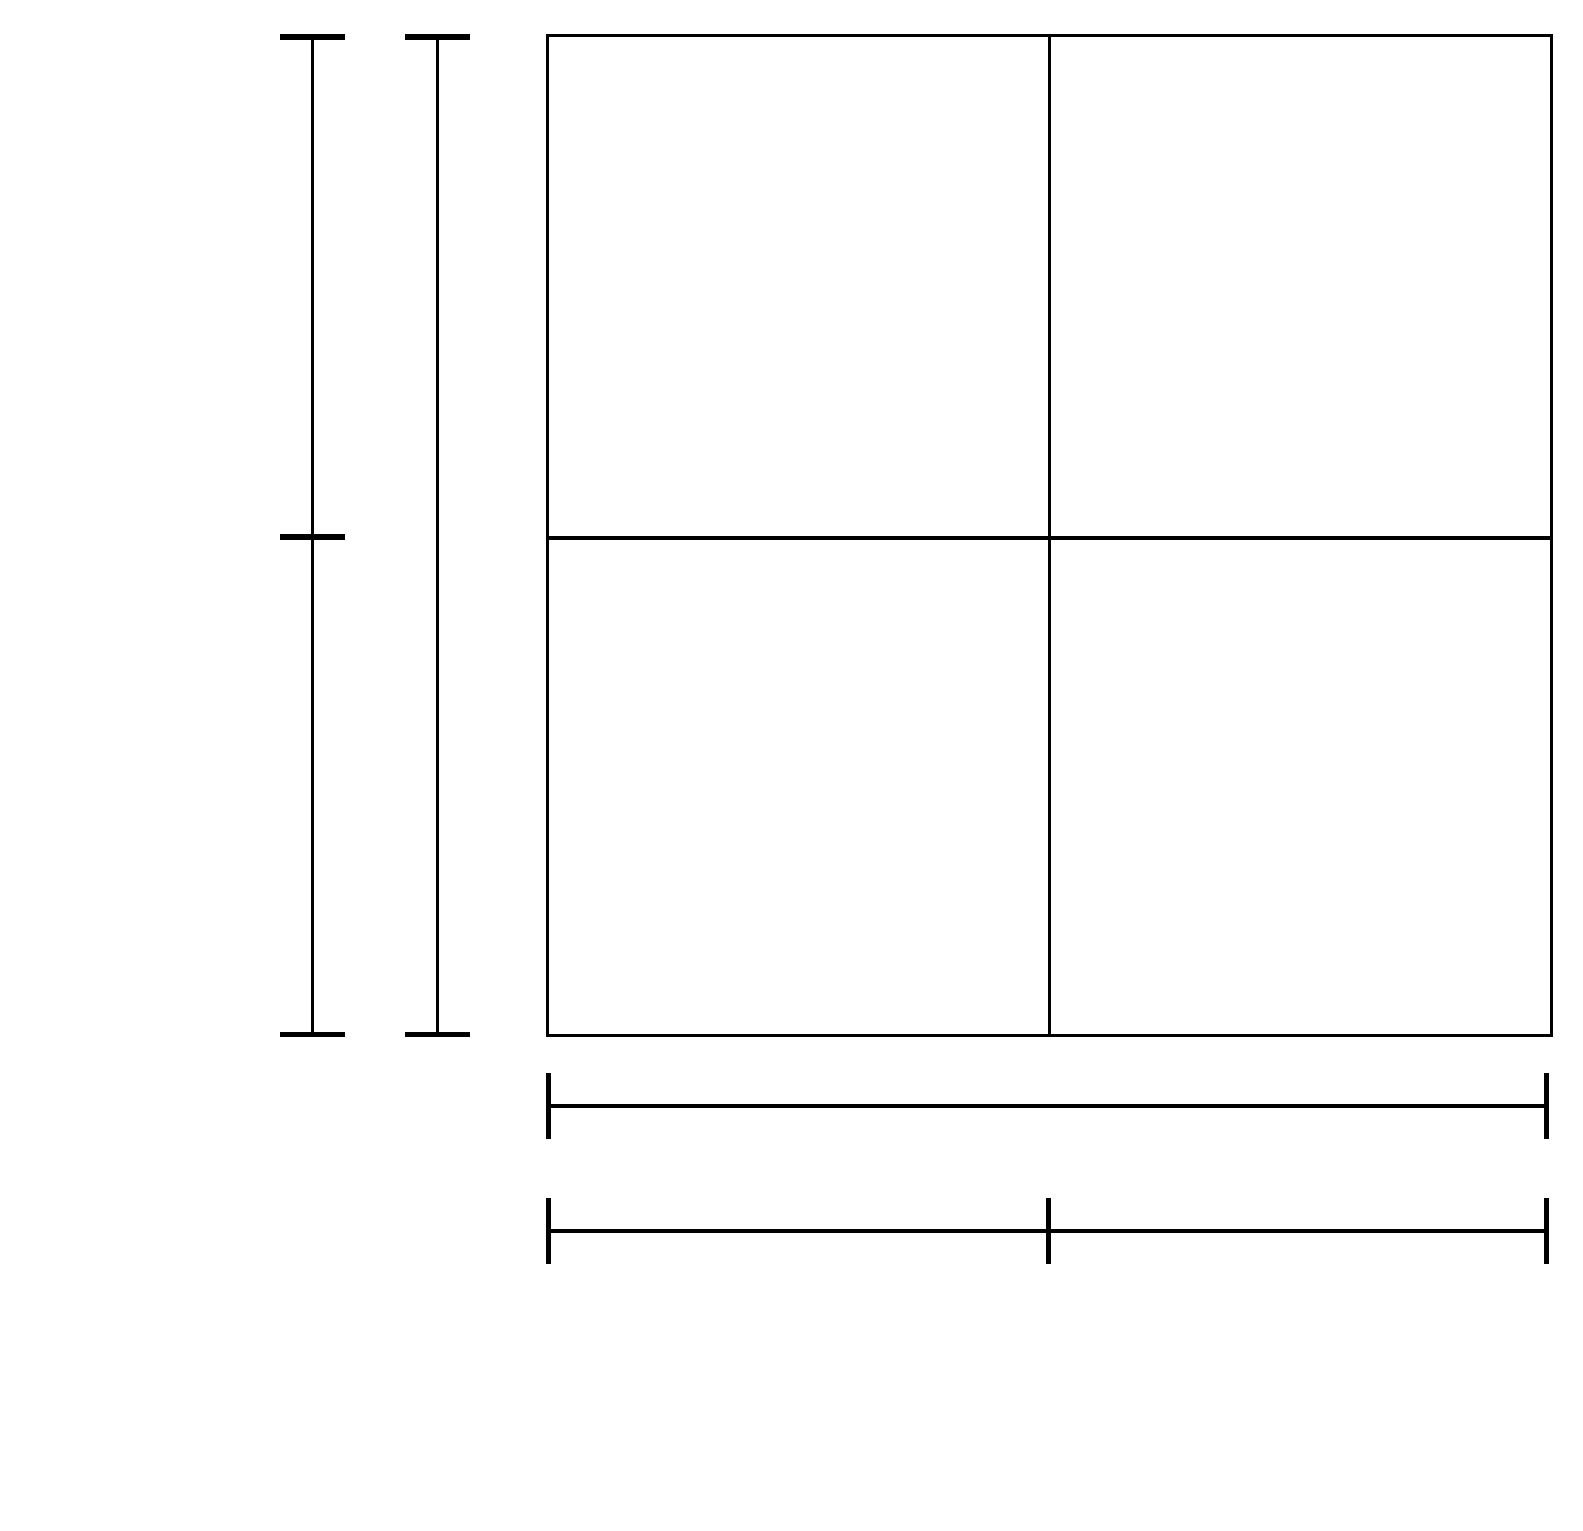
\includegraphics[width=\linewidth]{figures/fg-h2-matrix-2.pdf}
          \onslide<3>\centering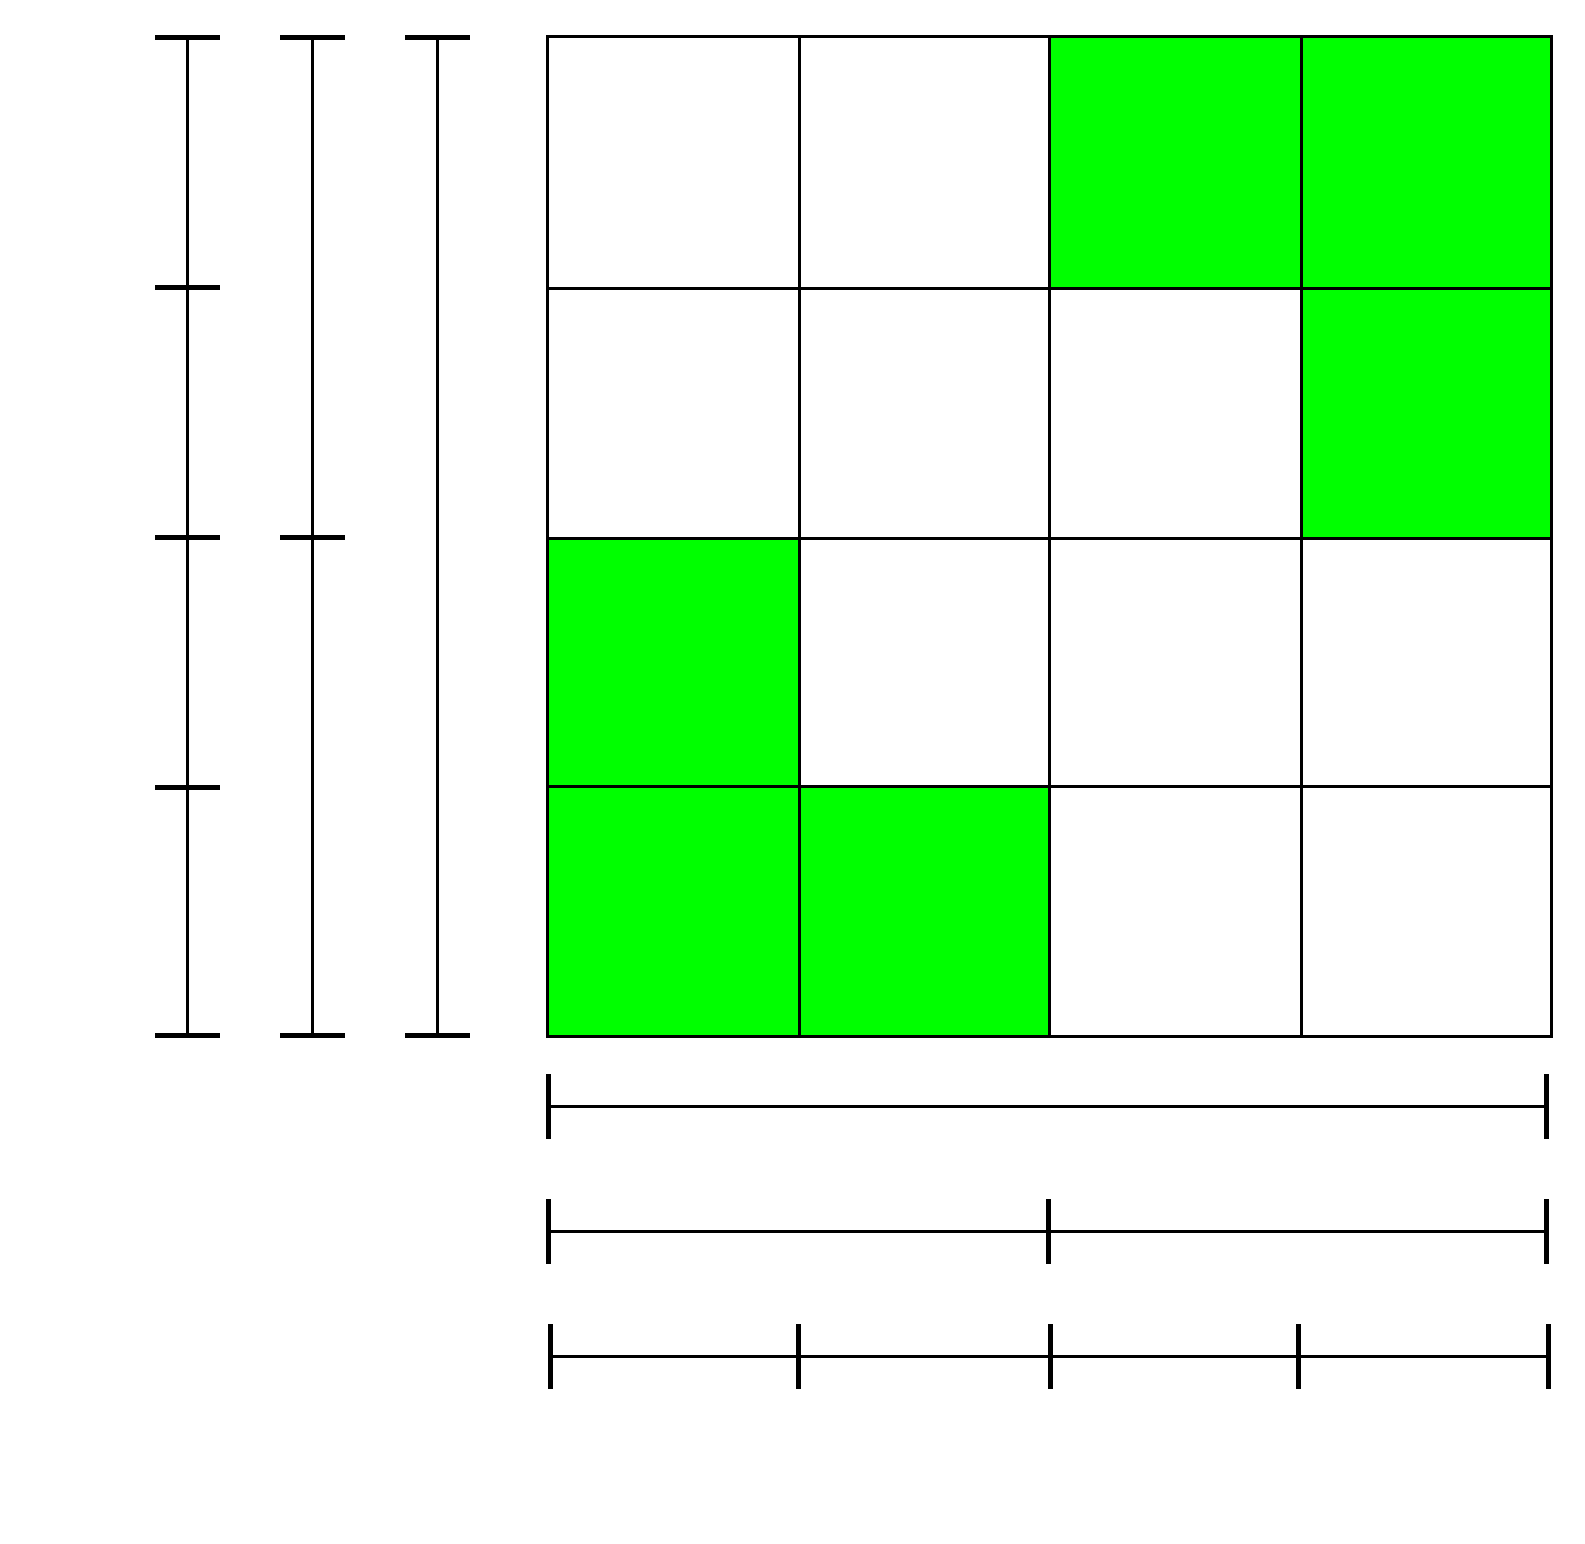
\includegraphics[width=\linewidth]{figures/fg-h2-matrix-3.pdf}
        \end{overprint}
      \end{figure}
    \column{.45\linewidth}
      \begin{itemize}
        \item \visible<1->{ Starte mit \( G \)}
        \item \visible<2->{ Unterteile unzulässige Untermatrizen}
      \end{itemize}
      
  \end{columns}

  \footnotesize
  \let\thefootnote\relax\footnote{Steffen B{\"o}rm.
  \href{https://books.google.de/books/about/Efficient_Numerical_Methods_for_Non_loca.html?id=awMabNC9DTkC&redir_esc=y}
  {\textit{Efficient numerical methods for non-local operators: \(
   \mathcal{H}^{2} \)-matrix compression, algorithms and analysis}}. Bd. 14.  
   European Mathematical Society, 2010.}
  \addtocounter{footnote}{-1}\let\thefootnote\svthefootnote\relax
  \normalsize
\end{frame}

\begin{frame}{\(\mathcal{H}^2\)-Matrizen}
  Teile \( G \) rekursiv in Untermatrizen bzgl. \textit{zulässiger} und
  \textit{unzulässiger} Unteräume \( \tau \times \sigma \) auf

  \begin{columns}
    \column{.45\linewidth}
      \begin{figure}
        \begin{overprint}
          \onslide<1>\centering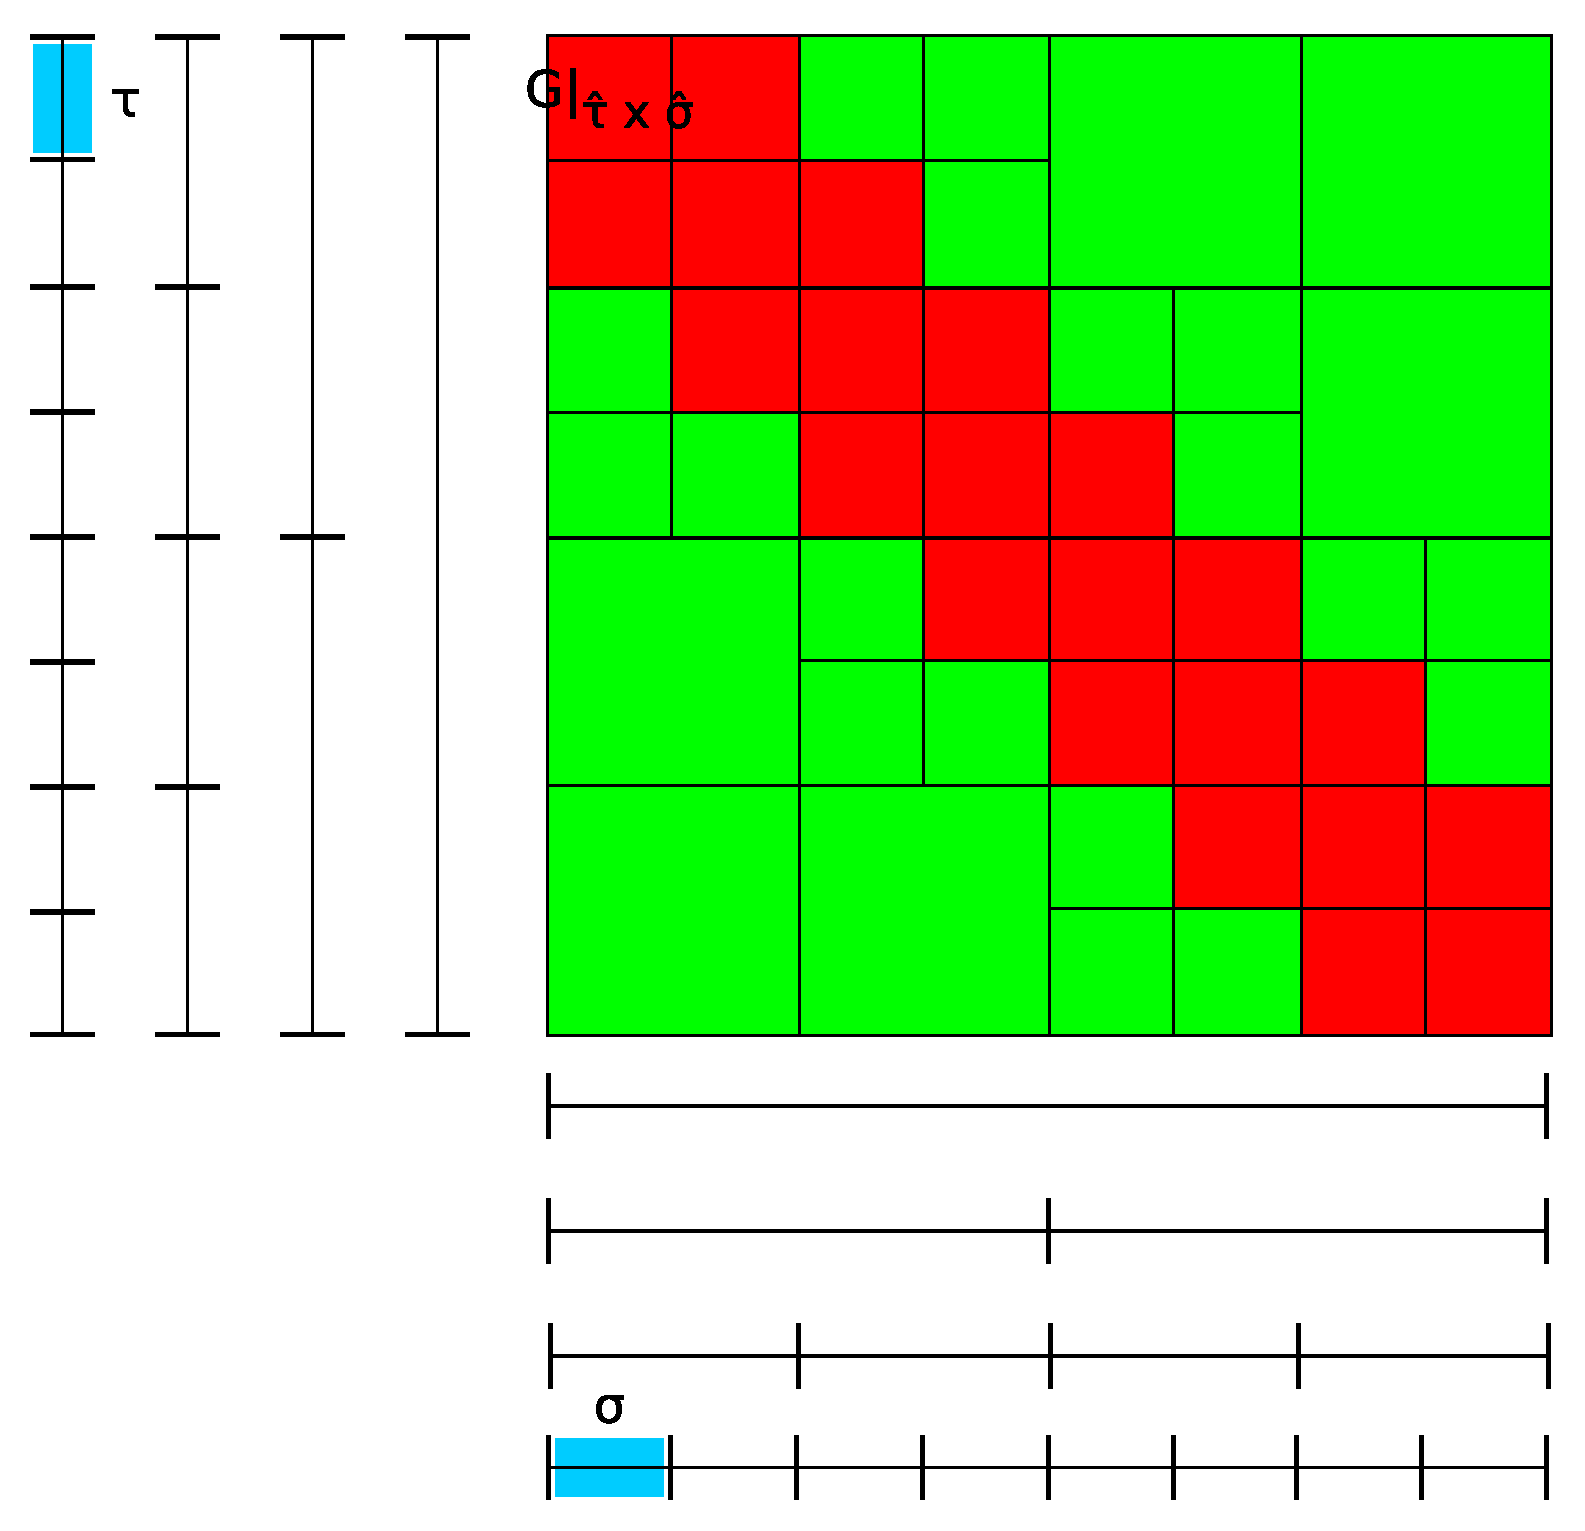
\includegraphics[width=\linewidth]{figures/fg-h2-matrix-4.pdf}
          \onslide<2>\centering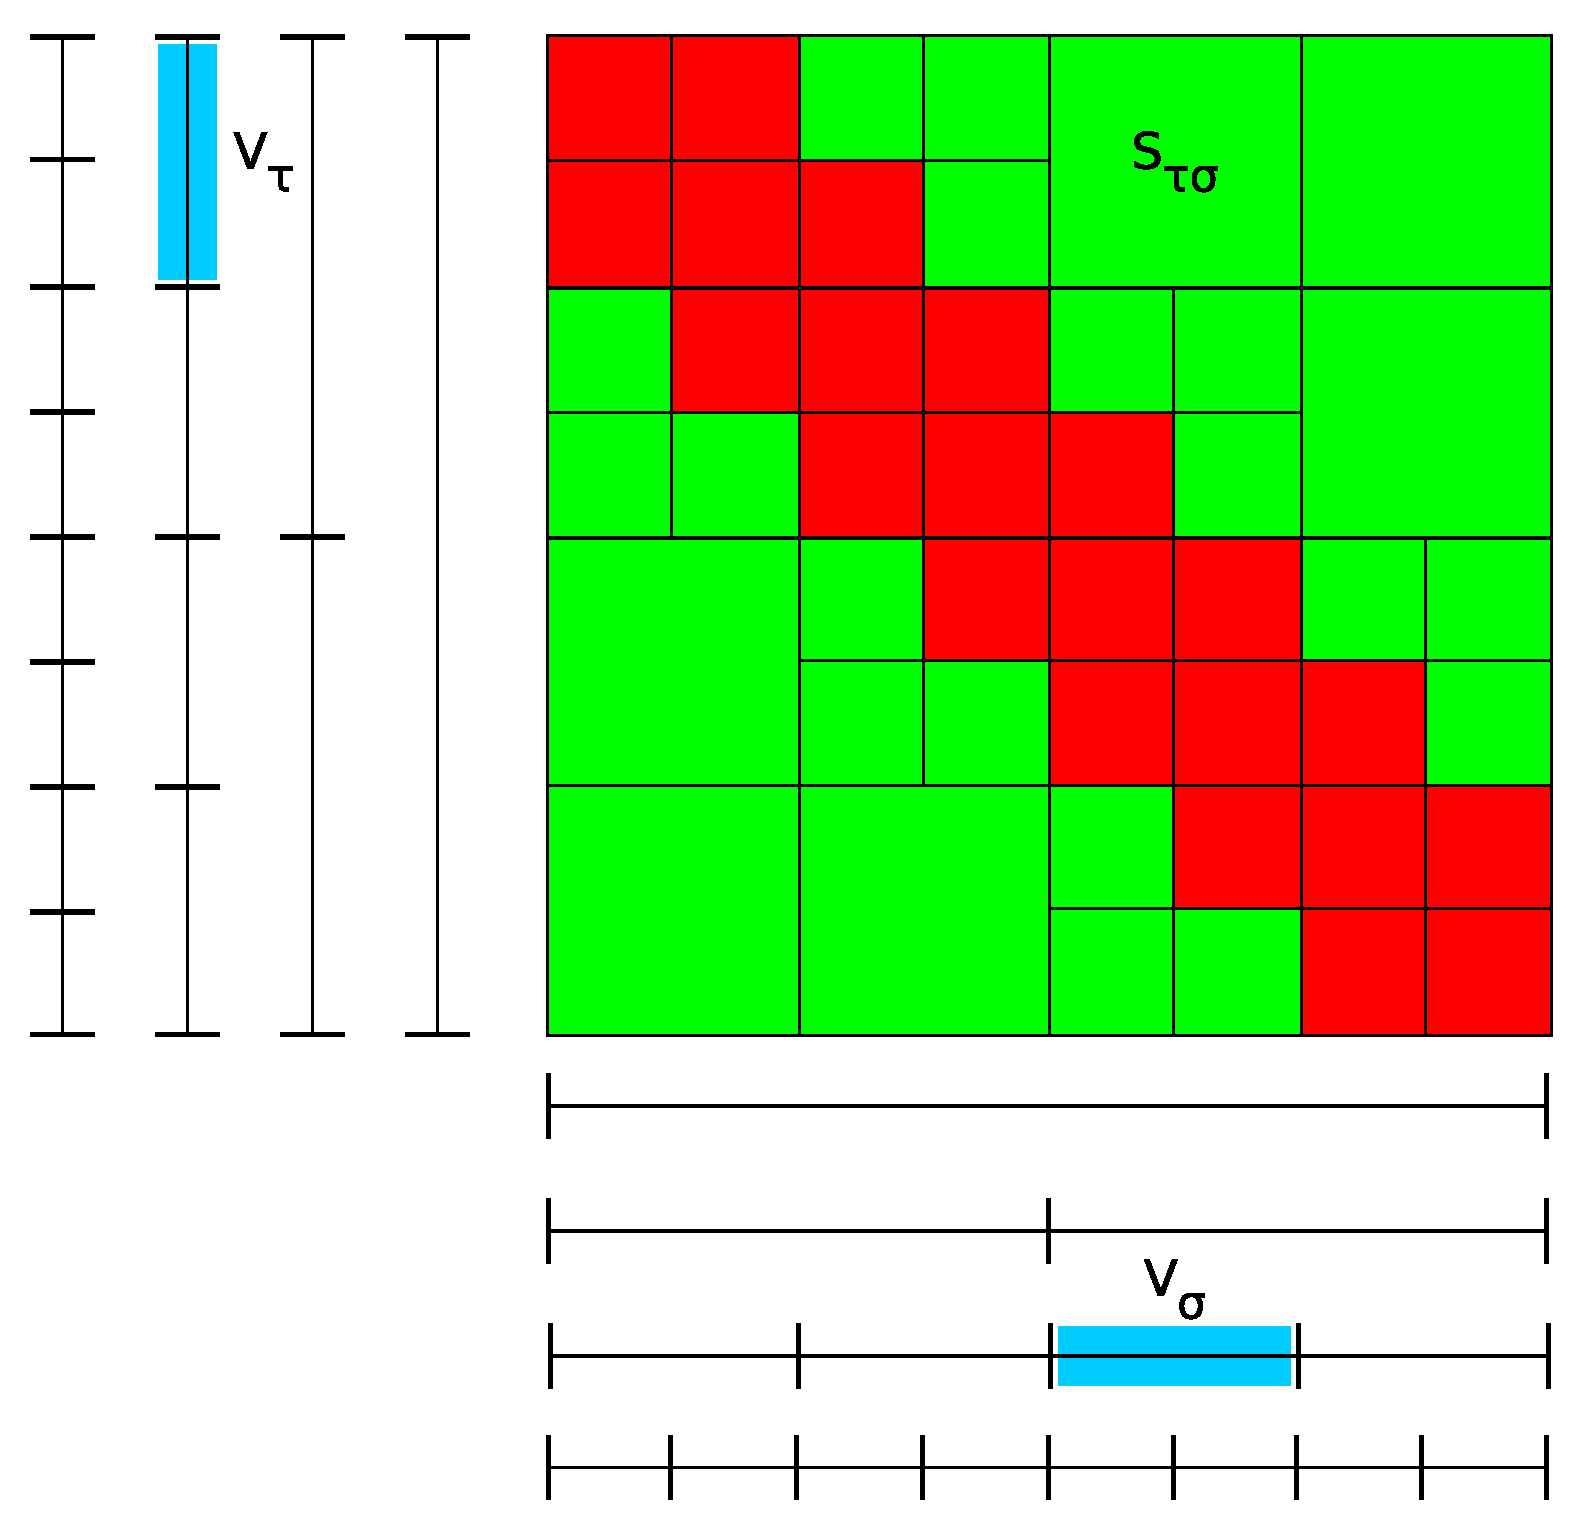
\includegraphics[width=\linewidth]{figures/fg-h2-matrix-5.pdf}
          \onslide<3>\centering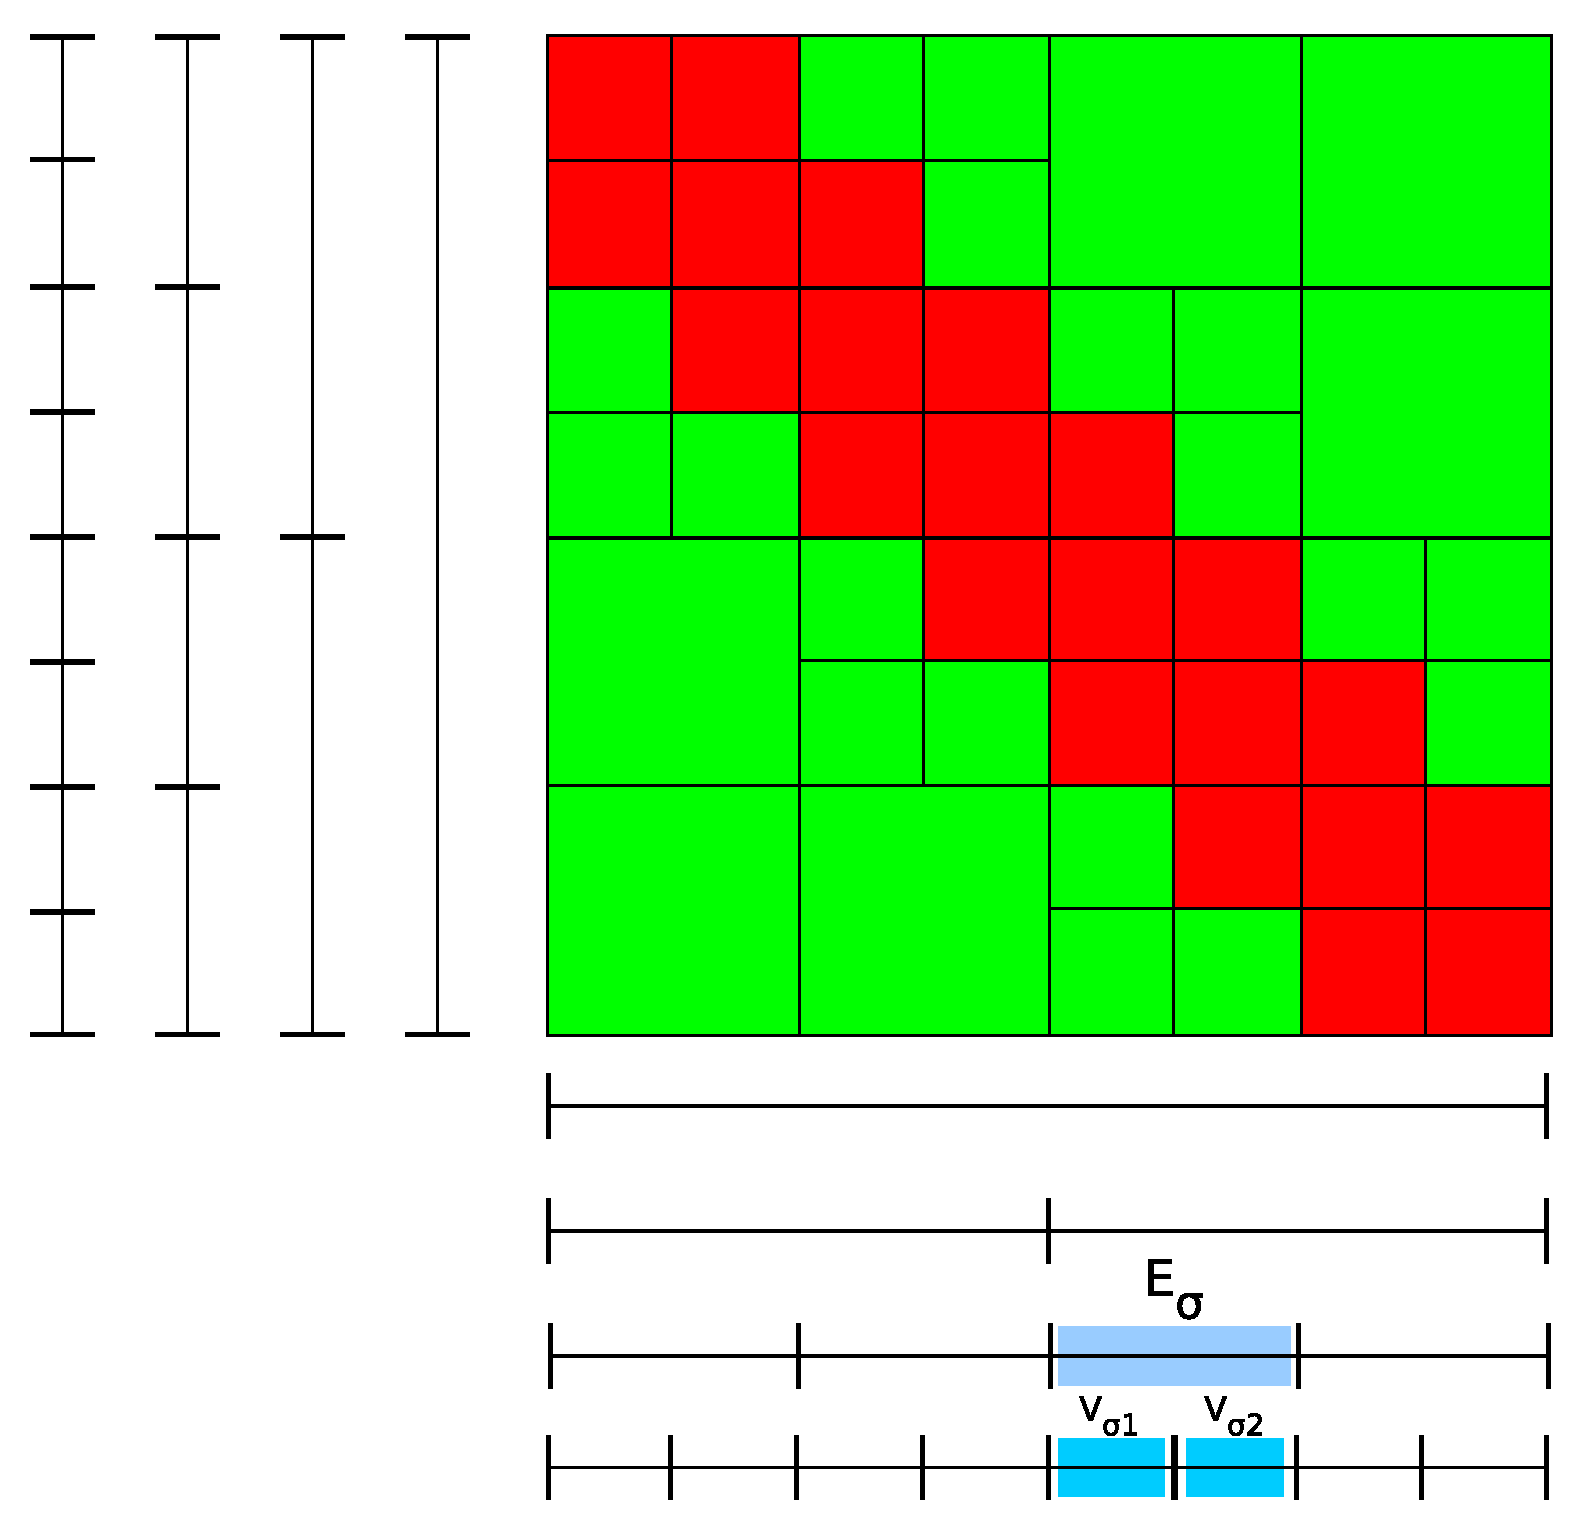
\includegraphics[width=\linewidth]{figures/fg-h2-matrix-6.pdf}
        \end{overprint}
      \end{figure}
    \column{.45\linewidth}
      \begin{itemize}
        \item \visible<1->{ Kleine unzulässige Untermatrizen werden nicht
          approximiert}
        \item \visible<2->{ Niedrigrangdarstellung \( G|_{\hat{\tau} \times \hat{\sigma}} \approx V_{\tau} S_{\tau\sigma} V_{\sigma}^{*} \) von
          zulässigen Untermatrizen}
        \item \visible<3->{ Verschachtelte Darstellung \( V_{\sigma} =
          \begin{pmatrix}
            V_{\sigma 1}E_{\sigma}|_{\sigma 1} \\
            V_{\sigma 2}E_{\sigma}|_{\sigma 2}
          \end{pmatrix} \) von Basismatrizen}
      \end{itemize}
  \end{columns}

  \footnotesize
  \let\thefootnote\relax\footnote{Steffen B{\"o}rm.
  \href{https://books.google.de/books/about/Efficient_Numerical_Methods_for_Non_loca.html?id=awMabNC9DTkC&redir_esc=y}
  {\textit{Efficient numerical methods for non-local operators: \(
   \mathcal{H}^{2} \)-matrix compression, algorithms and analysis}}. Bd. 14.  
   European Mathematical Society, 2010.}
  \addtocounter{footnote}{-1}\let\thefootnote\svthefootnote\relax
  \normalsize
\end{frame}

\begin{frame}{\(\mathcal{H}^2\)-Matrix-Vektor-Multiplikation}

  \begin{columns}
    \column{.3\linewidth}
      \( y|_{\hat{\tau}} := \overbrace{V_{\tau} \underbrace{S_{\tau \sigma}
        \overbrace{V_{\sigma}^{*}
        \textcolor{orange}{x|_{\hat{\sigma}}}}^{\textcolor{red}{\text{forward}}}}_{fastaddeval}}^{backward} \)
    \column{.3\linewidth}
      \( y|_{\hat{\tau}} := \overbrace{V_{\tau} \underbrace{S_{\tau \sigma}
         \textcolor{orange}{\hat{x}_\sigma}}_{\textcolor{red}{fastaddeval}}}^{backward} \)
    \column{.3\linewidth}
      \( y|_{\hat{\tau}} := \overbrace{V_{\tau}
         \textcolor{orange}{\hat{y}_\tau}}^{\textcolor{red}{backward}} \)
  \end{columns}
  \footnotesize
  \let\thefootnote\relax\footnote{Steffen B{\"o}rm.
  \href{https://books.google.de/books/about/Efficient_Numerical_Methods_for_Non_loca.html?id=awMabNC9DTkC&redir_esc=y}
  {\textit{Efficient numerical methods for non-local operators: \(
   \mathcal{H}^{2} \)-matrix compression, algorithms and analysis}}. Bd. 14.  
   European Mathematical Society, 2010.}
  \addtocounter{footnote}{-1}\let\thefootnote\svthefootnote\relax
  \normalsize
\end{frame}

\begin{frame}{\(\mathcal{H}^2\)-Matrix-Vektor-Multiplikation}
  \begin{columns}
    \column{.3\linewidth}
      \( y|_{\hat{\tau}} := \overbrace{V_{\tau} \underbrace{S_{\tau \sigma}
         \textcolor{orange}{\hat{x}_\sigma}}_{\textcolor{red}{fastaddeval}}}^{backward} \)
    \column{.6\linewidth}
          \begin{algorithm}[H]
            \SetKwProg{Proc}{}{}{}
            \Proc{fastaddeval \\ \quad \small{(\( \alpha, \ G, \ b = (t, s), \ x, \
                                                   \hat{x}, \, \textbf{var } y, \hat{y}
                                                \))}}
            {
              \uIf{\( b \in \mathcal{L}^{+}_{\mathcal{I} \times \mathcal{J}}
                   \)}
              {
                \( \hat{y}_{t} \leftarrow \hat{y}_{t} + \alpha S_{b}\hat{x}_{s}
                \) \;
              }
              \uElseIf{\( b \in\mathcal{L}^{-}_{\mathcal{I} \times
                          \mathcal{J}} \)}
              {
                \( y|_{\hat{t}} \leftarrow y|_{\hat{t}} + \alpha
                   N_{b}x|_{\hat{s}} \) \;
              }
              \Else{
                \ForAll{\( b' \in \text{sons}(b)\)}
                {
                  \small{\textit{fastaddeval\relax(}\( \alpha, \ G, \ b', \ x, \
                                                                  \hat{x}, \ y, \
                                                                  \hat{y} \)\textit{)} \;}
                }
              }
            }
          \end{algorithm}
  \end{columns}

  \footnotesize
  \let\thefootnote\relax\footnote{Steffen B{\"o}rm.
  \href{https://books.google.de/books/about/Efficient_Numerical_Methods_for_Non_loca.html?id=awMabNC9DTkC&redir_esc=y}
  {\textit{Efficient numerical methods for non-local operators: \(
   \mathcal{H}^{2} \)-matrix compression, algorithms and analysis}}. Bd. 14.  
   European Mathematical Society, 2010.}
  \addtocounter{footnote}{-1}\let\thefootnote\svthefootnote\relax
  \normalsize
\end{frame}

\section{Sauter-Schwab Quadratur}

\begin{frame}{Sauter-Schwab Quadratur}
  \begin{itemize}
    \item Vier Fälle von Integralen, abhängig von den entsprechenden 
          Dreieckspaaren \( \Delta_{i}, \ \Delta_{j} \) der Triangulation:
    \begin{enumerate}
        \item \( \Delta_{i} \) und \( \Delta_{j} \) sind disjunkt, also \(
                 \Delta_{i} \cap \Delta_{j} = \emptyset \).
        \item \( \Delta_{i} \) und \( \Delta_{j} \) teilen sich einen Vertex \(
                 v \in \mathbb{R}^{d} \), also \( \Delta_{i} \cap \Delta_{j} = 
                 \{ v \} \).
        \item \( \Delta_{i} \) und \( \Delta_{j} \) teilen sich eine Kante
              \( \{ v_{1}, \ v_{2} \} \in \mathbb{R}^{d} \times \mathbb{R}^{d} 
              \), also \( \Delta_{i} \cap \Delta_{j} = \{ v_{1}, \ v_{2} \} \).
        \item \( \Delta_{i} \) und \( \Delta_{j} \) sind identisch, also \(
                 \Delta_{i} = \Delta_{i} \cap \Delta_{j} = \Delta_{j} \).
    \end{enumerate}
    \item Permutation der Eckpunkte und approximiere das Integral dann durch
          eine gewichtete Summe von Kernauswertungen
  \end{itemize}

  \footnotesize
  \let\thefootnote\relax\footnote{S. A. Sauter und C. Lage.
  \href{https://link.springer.com/article/10.1007\%2Fs00211-015-0757-y}{
  ``On the efficient computation of singular and nearly singular surface 
  integrals arising in 3D-Galerkin BEM''}. In:   \textit{Zeitschrift f\"ur 
  angewandte Mathematik und Mechanik } 76 (1996), S. 273-275.}
  \addtocounter{footnote}{-1}\let\thefootnote\svthefootnote\relax
  \normalsize
\end{frame}

\section{GCA-Methode}

\begin{frame}{GCA-Methode}
  \begin{itemize}
    \item Sei ein zulässiger Block \(b = (\tau, \ \sigma)\) gegeben
    \item Algebraische Interpolation in zulässigen Blättern
    \begin{itemize}
      \item Greens zweite Identität, Quadratur und adaptive Kreuzapproximation
            (adaptive cross approximation [ACA])
      \item \visible<2->{\(\mathfrak{I}_{\tau} = V_{\tau}P_{\tau}, \qquad
                           \mathfrak{I}_{\sigma} = W_{\sigma}P_{\sigma}\)}
      \item \visible<2->{\(V_{\tau} \in \mathbb{R}^{\tau \times \tilde{\tau}},
                           \qquad W_{\sigma} \in \mathbb{R}^{\sigma \times
                           \tilde{\sigma}}\): \glqq Interpolationspolynome\grqq}
      \item \visible<2->{\(P_{\tau} \in \mathbb{R}^{\tilde{\tau} \times \tau},
                           \qquad P_{\sigma} \in \mathbb{R}^{\tilde{\sigma}
                           \times \sigma}\): \glqq Interpolationpunkte\grqq}
      \item \visible<2->{\(\tilde{\tau} \subseteq \tau, \qquad \tilde{\sigma}
                           \subseteq \sigma\)}
      \item \visible<3->{\(G|_{\tau \times \sigma} \approx
                           \mathfrak{I}_{\tau} G|_{\tau \times \sigma}
                           \mathfrak{I}_{\sigma}^{*} =
                           V_{\tau} G|_{\tilde{\tau} \times \tilde{\sigma}}
                           W_{\sigma}^{*}\)}
    \end{itemize}
    \item \visible<4->{Innere Knoten: Greens zweite Identität auf die von den Söhnen ausgewählten Basisfunktionen und ACA}
  \end{itemize}

  \footnotesize
  \let\thefootnote\relax\footnote{Steffen Börm und Sven Christophersen.
  \href{https://link.springer.com/article/10.1007\%2Fs00211-015-0757-y}{
  ``Approximation of integral operators by Green quadrature and nested cross 
  approximation''}. In: \textit{Numerische Mathematik} 133.3 (2016), S. 
  409-442, 2016.}
  \addtocounter{footnote}{-1}\let\thefootnote\svthefootnote\relax
  \normalsize
\end{frame}

\section{GPUs}

\begin{frame}{GPUs}
  \begin{columns}
    \column{0.44\linewidth}
      \begin{itemize}
        \item Graphics Processing Units (GPUs) sind ein auf Computergrafik
              spezialisierte Prozessoren
        \begin{itemize}
          \item Schnelle Gleitkomma-Operationen
          \item Vektorisierte Architektur
        \end{itemize}
        \item Entwicklung von GPUs durch Videospielindustrie stark
              vorangetrieben
        \item Sehr günstig dank Massenproduktion
      \end{itemize}
    \column{0.46\linewidth}
      \begin{figure}
        \centering
        \includegraphics[width=\linewidth]{figures/fg-flops.png}
        \caption{Theoretische Verarbeitungsgeschwindigkeit von
                 Gleitkomma-Operationen verschiedener
                 Architekturen}
      \end{figure}
  \end{columns}

  \footnotesize
  \let\thefootnote\relax\footnote{Nalan Ba\c{s}t{\"u}rk u.\,a.
  \href{https://www.researchgate.net/publication/292514527_Parallelization_Experience_with_Four_Canonical_Econometric_Models_Using_ParMitISEM}{
  ``Parallelization experience with four canonical econometric models using ParMitISEM''}. In: \textit{Econometrics} 4.1 (2016), S. 11.}
  \addtocounter{footnote}{-1}\let\thefootnote\svthefootnote\relax
  \normalsize
\end{frame}

\begin{frame}{GPUs}
  \begin{figure}
    \centering
    \includegraphics[width=\linewidth]{figures/fg-gpu_architecture.pdf}
    \caption{Architektur einer Grafikkarte}
  \end{figure}

  \footnotesize
  \let\thefootnote\relax\footnote{Sunpyo Hong und Hyesoon Kim.
  \href{https://link.springer.com/article/10.1007\%2Fs00211-015-0757-y}{
  ``An analytical model for a GPU architecture with memory-level and thread-level parallelism awareness''}. In:   \textit{ACM SIGARCH Computer 
  Architecture News}. Bd. 37. 3. 2009, S. 152-163.}
  \addtocounter{footnote}{-1}\let\thefootnote\svthefootnote\relax
  \normalsize
\end{frame}

\section{OpenCL}

\begin{frame}{OpenCL}
  \begin{itemize}
    \item Framework zum Programmieren von/auf unterschiedlichen
          Hardware-Architekturen
    \begin{itemize}
      \item Field Programmable Gate Arrays (FPGAs)
      \item Digitaler Signalprozessoren (DSPs)
      \item CPUs
      \item GPUs
    \end{itemize}
  \end{itemize}

  \footnotesize
  \let\thefootnote\relax\footnote{Alex Bourd. \href{https://www.khronos.org/registry/OpenCL/specs/opencl-2.2.pdf}{\textit{The OpenCL Specifictaion}}. 2.2. Document Revision: v2.2-3. Khronos OpenCL Working Group. Mai 2017.}
  \addtocounter{footnote}{-1}\let\thefootnote\svthefootnote\relax
  \normalsize
\end{frame}

\begin{frame}{OpenCL}
  \begin{figure}
    \centering
    \includegraphics[width=.75\linewidth]{figures/fg-opencl-platform-model.pdf}
    \caption{OpenCL-Plattformmodell}
  \end{figure}

  \footnotesize
  \let\thefootnote\relax\footnote{Alex Bourd. \href{https://www.khronos.org/registry/OpenCL/specs/opencl-2.2.pdf}{\textit{The OpenCL Specifictaion}}. 2.2. Document Revision: v2.2-3. Khronos OpenCL Working Group. Mai 2017.}
  \addtocounter{footnote}{-1}\let\thefootnote\svthefootnote\relax
  \normalsize
\end{frame}

\begin{frame}{OpenCL}
  \begin{figure}
    \centering
    \includegraphics[width=.6\linewidth]{figures/fg-opencl-memory-model.pdf}
    \caption{Das Speichermodell von OpenCL}
  \end{figure}

  \footnotesize
  \let\thefootnote\relax\footnote{Alex Bourd. \href{https://www.khronos.org/registry/OpenCL/specs/opencl-2.2.pdf}{\textit{The OpenCL Specifictaion}}. 2.2. Document Revision: v2.2-3. Khronos OpenCL Working Group. Mai 2017.}
  \addtocounter{footnote}{-1}\let\thefootnote\svthefootnote\relax
  \normalsize
\end{frame}

\begin{frame}{OpenCL}
  \begin{figure}
    \centering
    \includegraphics[width=.7\linewidth]{figures/fg-opencl-execution-model.pdf}
    \caption{Das Ausführungsmodell von OpenCL}
  \end{figure}

  \footnotesize
  \let\thefootnote\relax\footnote{Alex Bourd. \href{https://www.khronos.org/registry/OpenCL/specs/opencl-2.2.pdf}{\textit{The OpenCL Specifictaion}}. 2.2. Document Revision: v2.2-3. Khronos OpenCL Working Group. Mai 2017.}
  \addtocounter{footnote}{-1}\let\thefootnote\svthefootnote\relax
  \normalsize
\end{frame}

\begin{frame}[fragile]{OpenCL}
  \begin{lstlisting}[style=CStyle]
  kernel void vec_inc(const size_t n,
                      global float *a,
                      const float b)
  {
    const size_t gid = get_global_id(0);

    if(gid >= n)
      return;

    a[gid] += b;
  }
  \end{lstlisting}
\end{frame}
\section{3-Phasen-fastaddeval}

\begin{frame}{Idee}
  \begin{columns}
    \column{.5\linewidth}
      \begin{itemize}
        \item Berechne reproduzierbare Matrizen nur bei Bedarf:
        \item Fernfeldmatrizen \(S_{b} =
              G|_{\tilde{\tau} \times \tilde{\sigma}}\)
        \begin{itemize}
          \item Permutierte Eintr\"age der Galerkin-Diskretisierung
          \item Eintr\"age bestehen nur aus einem Integraltypen
        \end{itemize}
        \item Nahfeldmatrizen \( G|_{\hat{\tau} \times \hat{\sigma}} \)
        \begin{itemize}
          \item Eintr\"age der Galerkin-Diskretisierung
          \item Eintr\"age bestehen aus allen Integraltypen
        \end{itemize}
      \end{itemize}
    \column{.5\linewidth}
      \begin{algorithm}[H]
        \SetKwProg{Proc}{}{}{}
        \Proc{fastaddeval\relax(\( \alpha, \ G, \ x, \
                                              \hat{x}, \, \textbf{var } y,
                                              \hat{y} \))}
        {
          \ForAll{ \( b \in \mathcal{L}^{+}_{\mathcal{I} \times \mathcal{J}}
                   \) }
          {
            \( \hat{y}_{t} \leftarrow \hat{y}_{t} + \alpha G|_{\tilde{\tau}
               \times \tilde{\sigma}}\hat{x}_{s} \) \;
          }
          \ForAll{\( b \in\mathcal{L}^{-}_{\mathcal{I} \times
                     \mathcal{J}} \)}
          {
            \( y|_{\hat{t}} \leftarrow y|_{\hat{t}} + \alpha
               G|_{\hat{\tau} \times \hat{\sigma}}x|_{\hat{s}} \) \;
          }
        }
      \end{algorithm}
  \end{columns}
\end{frame}

\begin{frame}{Vorbereitung}\vfill
  \begin{figure}
    \begin{overprint}
      \onslide<1>
        \centering
        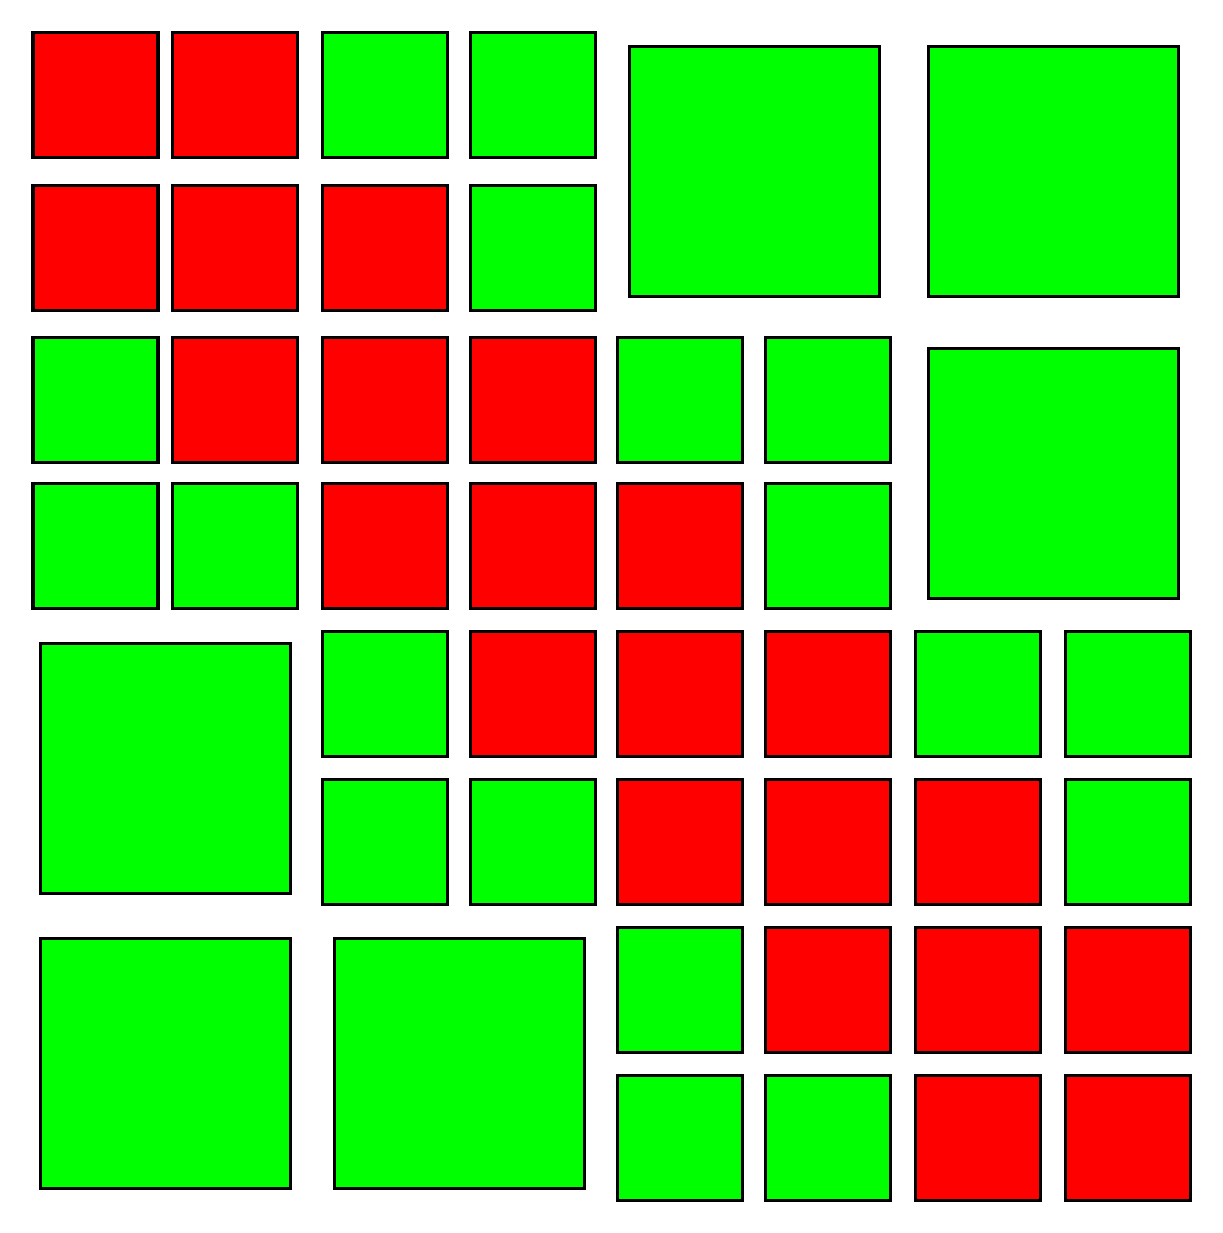
\includegraphics[width=.66\linewidth]{figures/fg-h2-matrix-block.pdf}
        \caption{Betrachte jede Blockmatrix einzeln}
      \onslide<2>
        \centering
        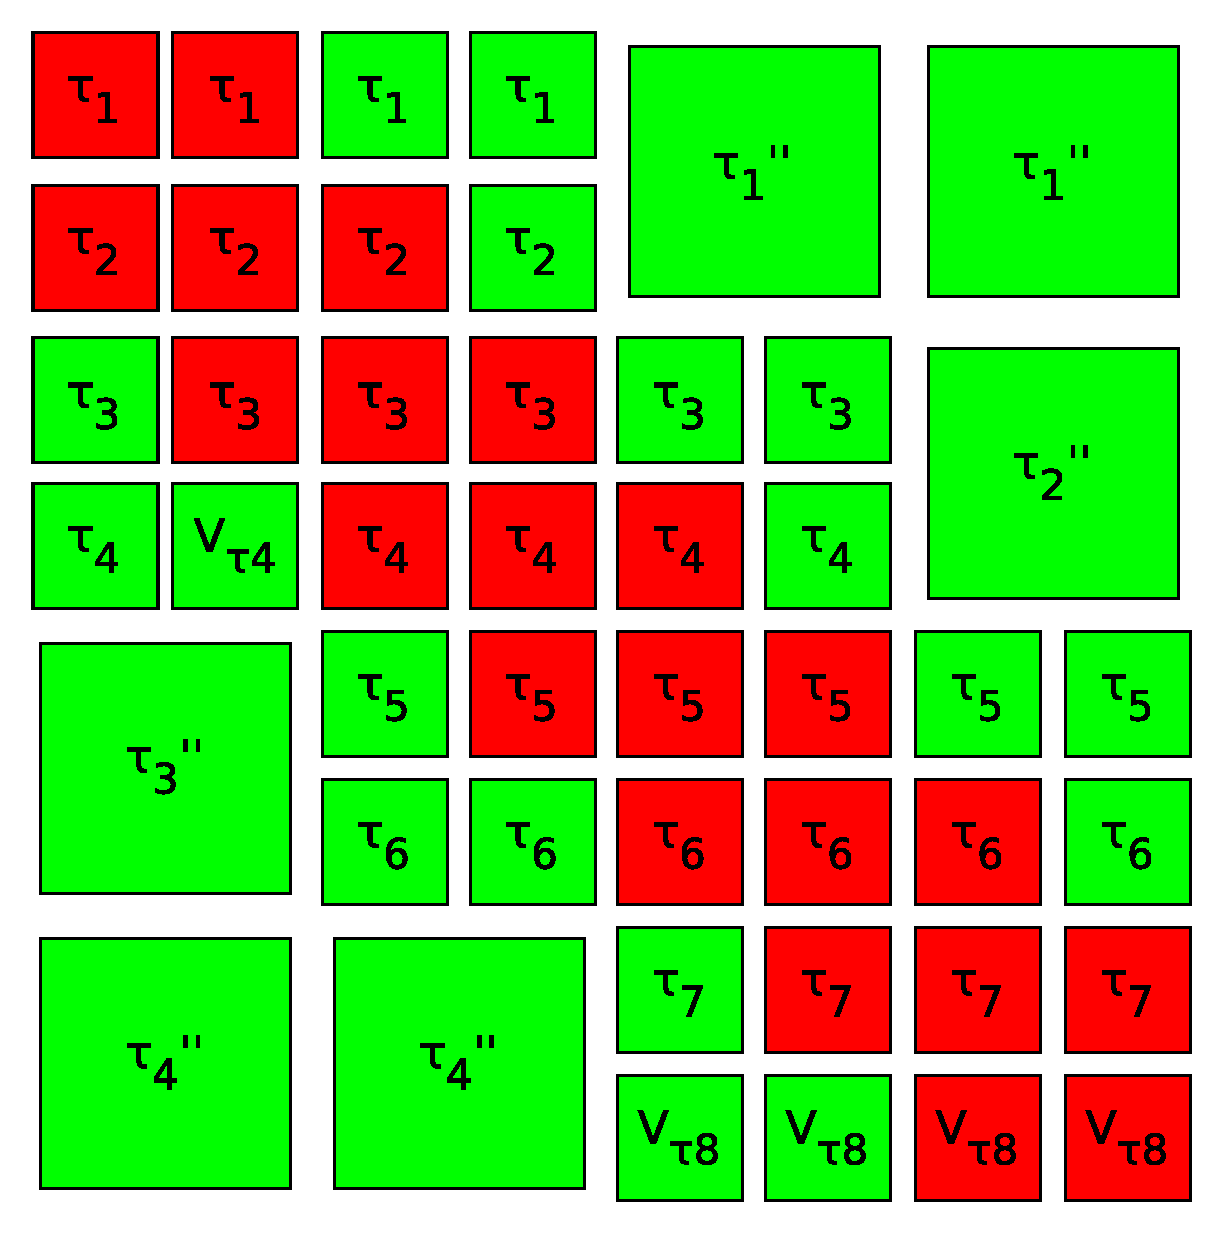
\includegraphics[width=.66\linewidth]{figures/fg-h2-matrix-block-labled.pdf}
        \caption{Kennzeichne die Blockmatrizen mit dem zust\"andigen Zeilencluster}
      \onslide<3>
        \centering
        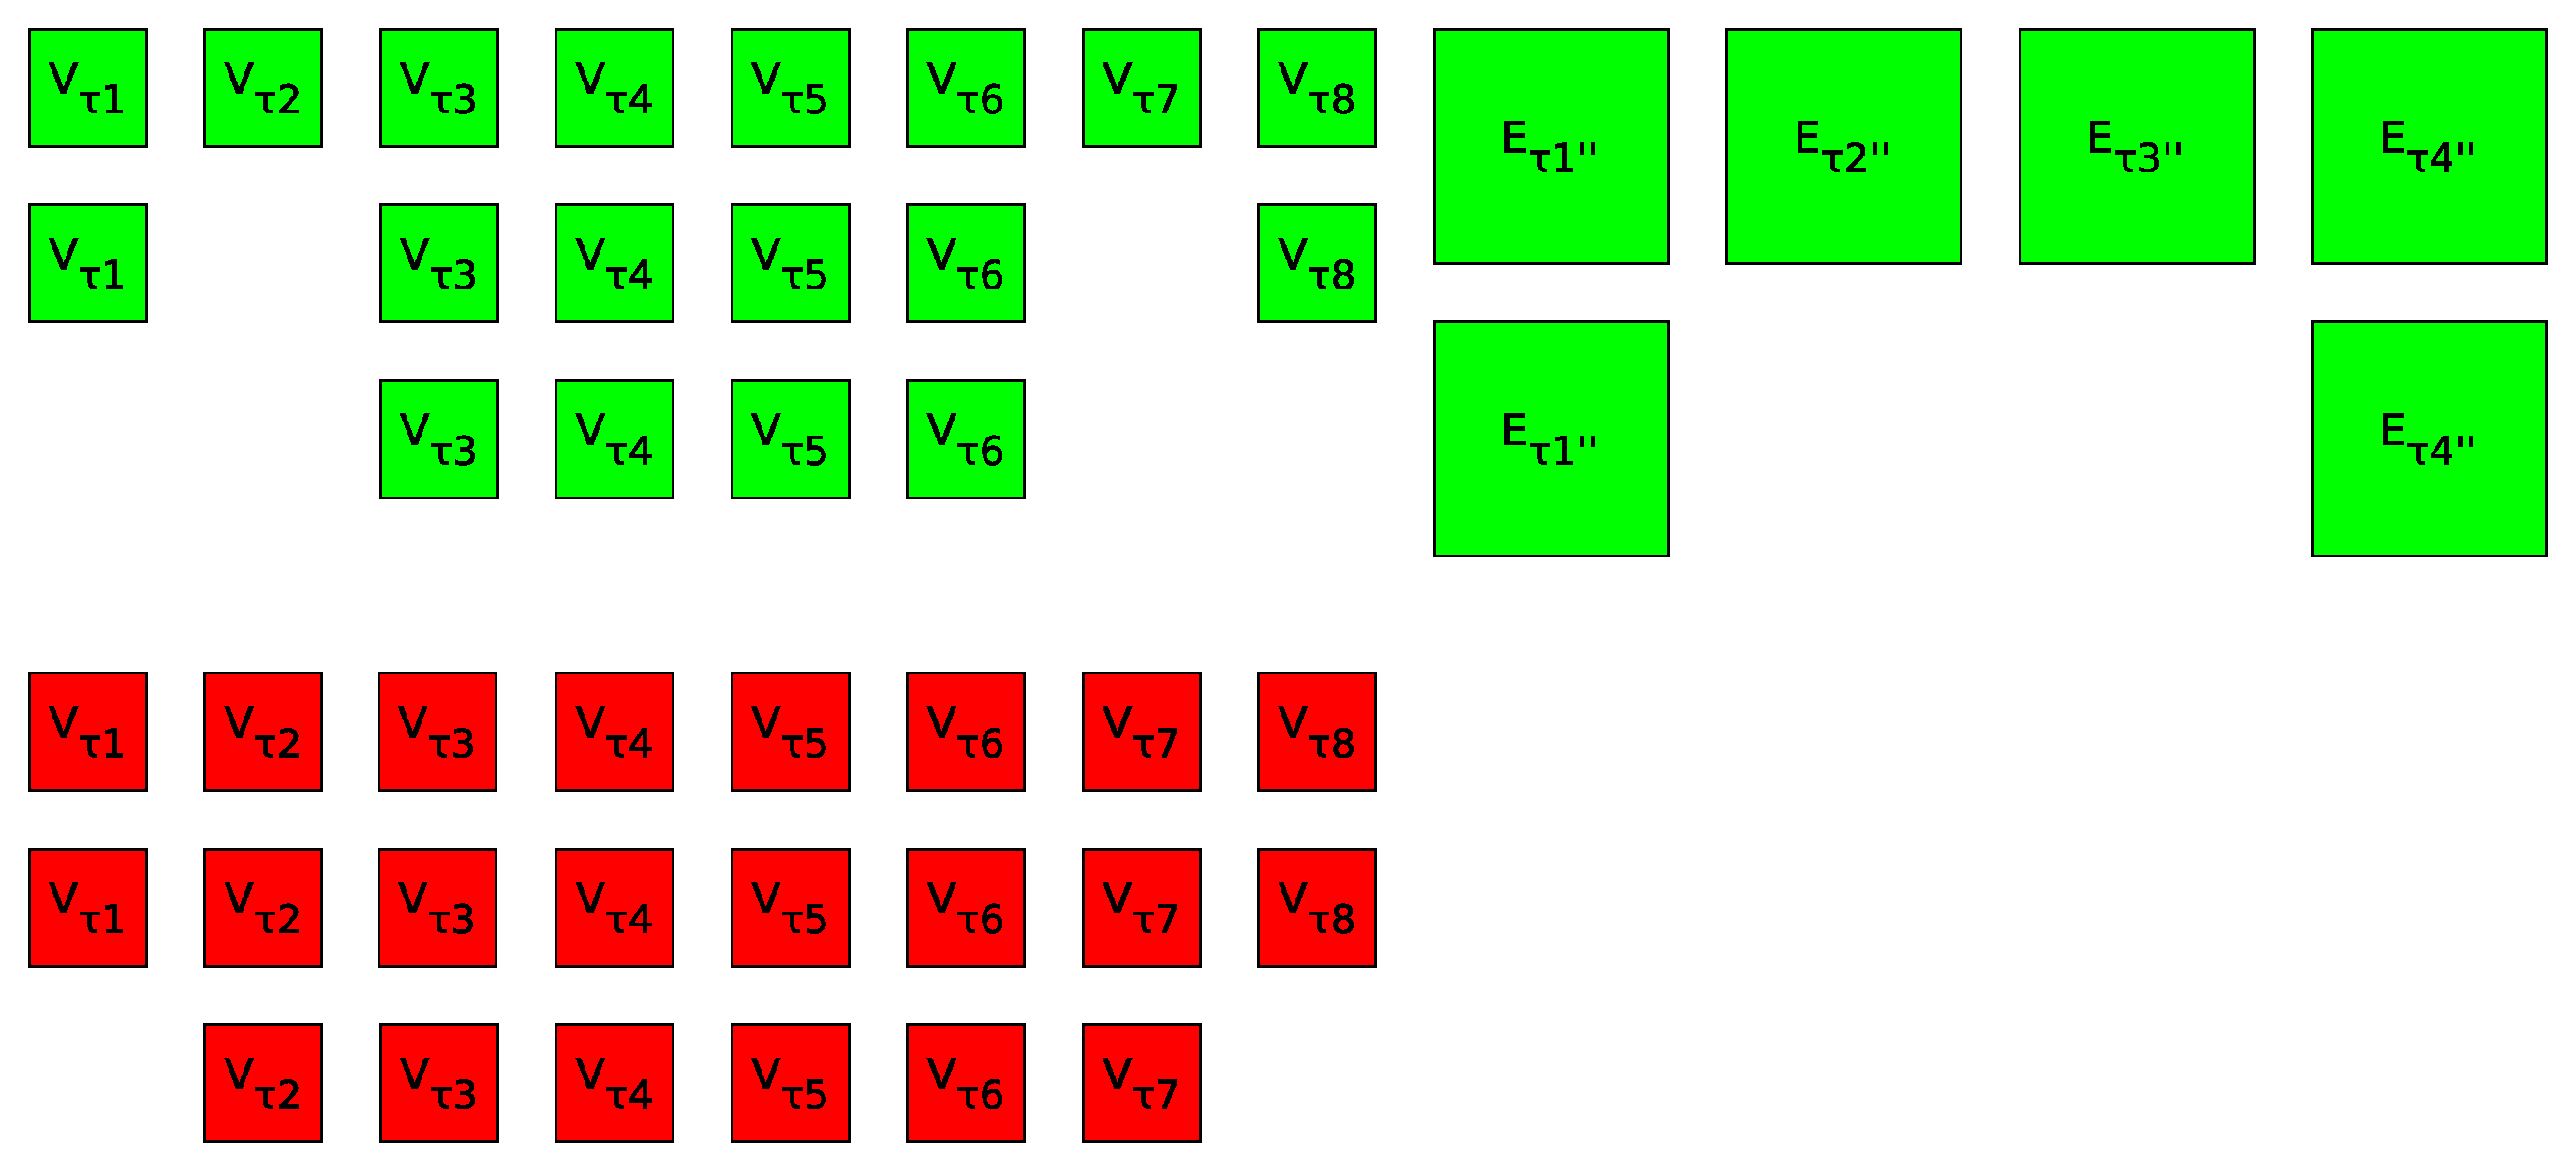
\includegraphics[width=\linewidth]{figures/fg-h2-matrix-block-orderd.pdf}
        \caption{Gruppierung von Blockmatrizen nach Fern- bzw. Nahfeld und nach
                 zust\"andigem Zeilencluster}
    \end{overprint}
  \end{figure}
\end{frame}

\begin{frame}{1. Phase (Fernfeld)}
  \begin{figure}
    \begin{overprint}
      \onslide<1>
        \centering
        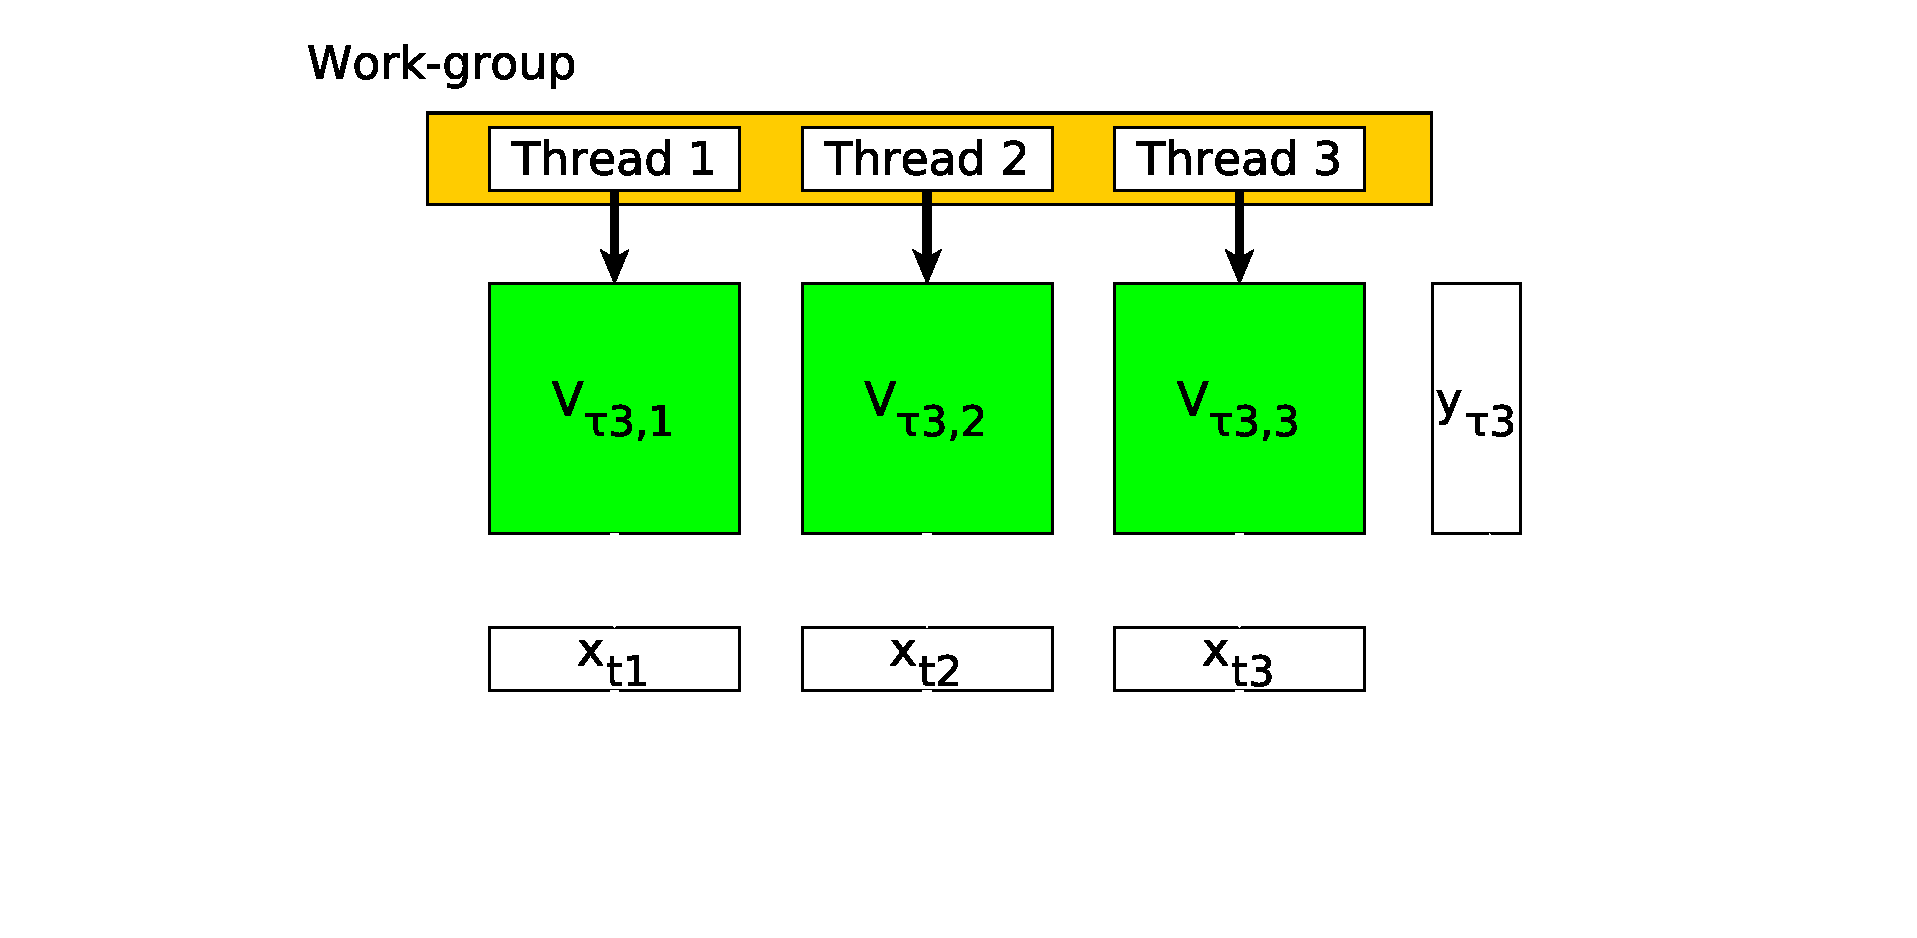
\includegraphics[width=\linewidth]{figures/fg-ff-initial-situation.pdf}
        \caption{Ausgangssituation einer OpenCL-Work-Group in der 1. Phase.}
      \onslide<2>
        \centering
        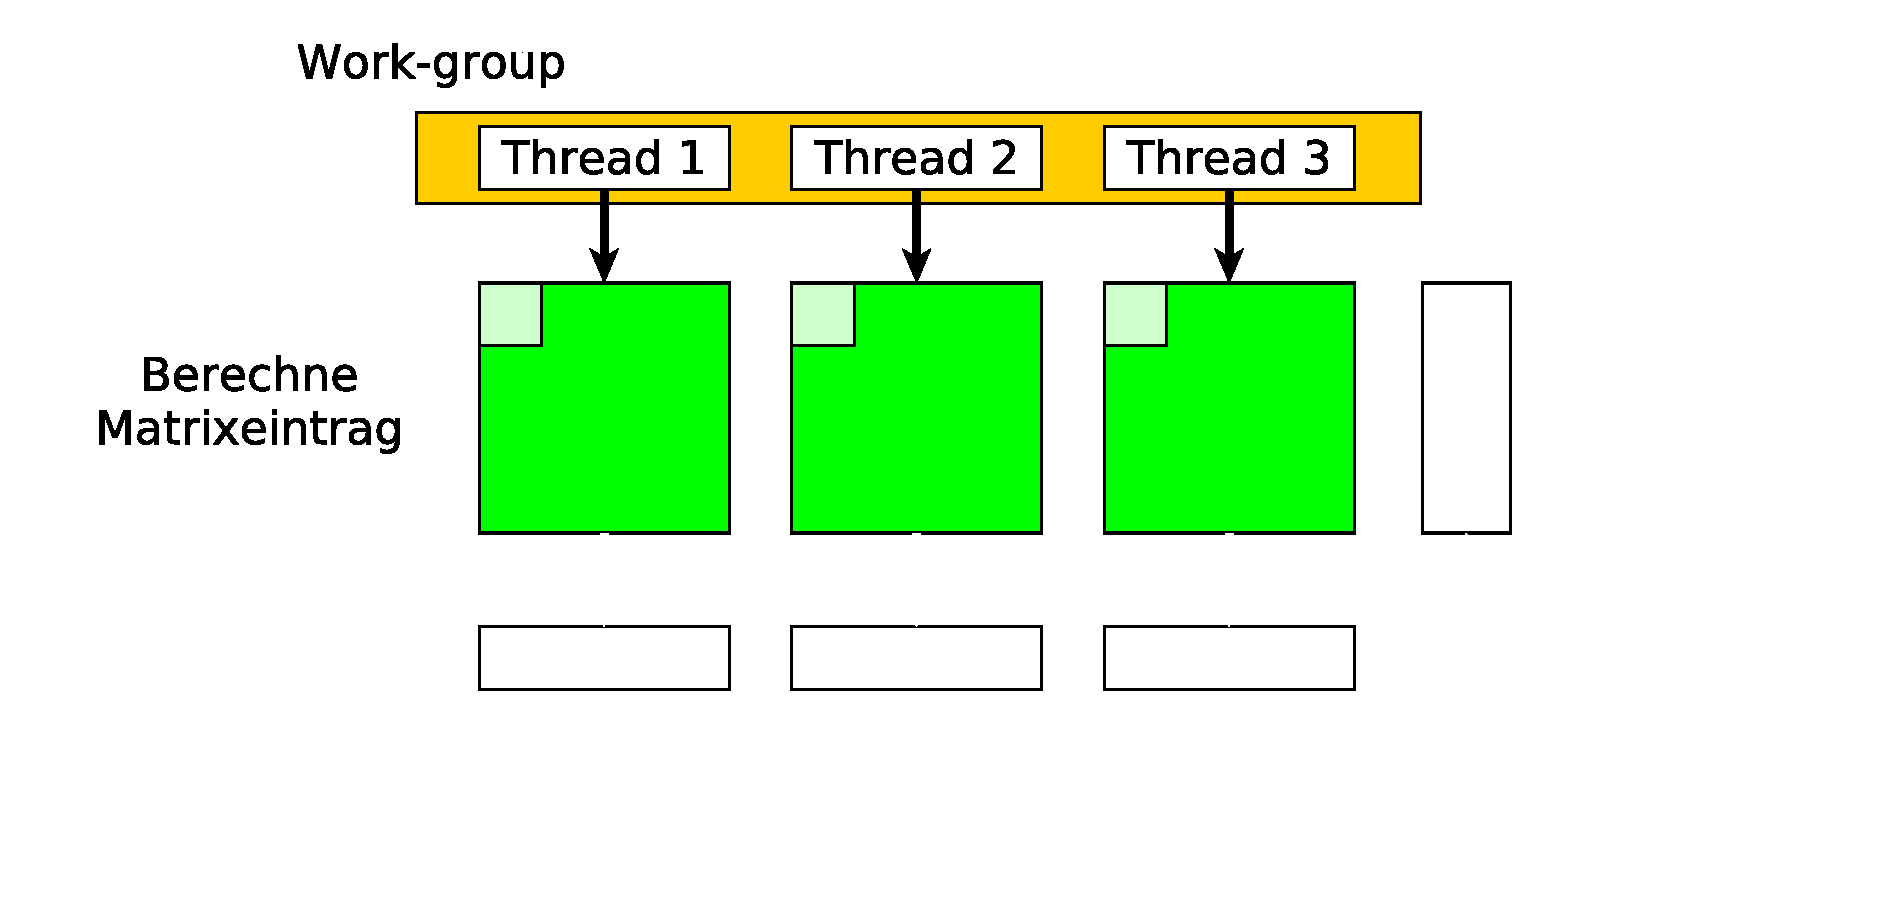
\includegraphics[width=\linewidth]{figures/fg-ff-compute-matrix-entry.pdf}
        \caption{Berechne den ersten Eintrag einer Matrixzeile.}
      \onslide<3>
        \centering
        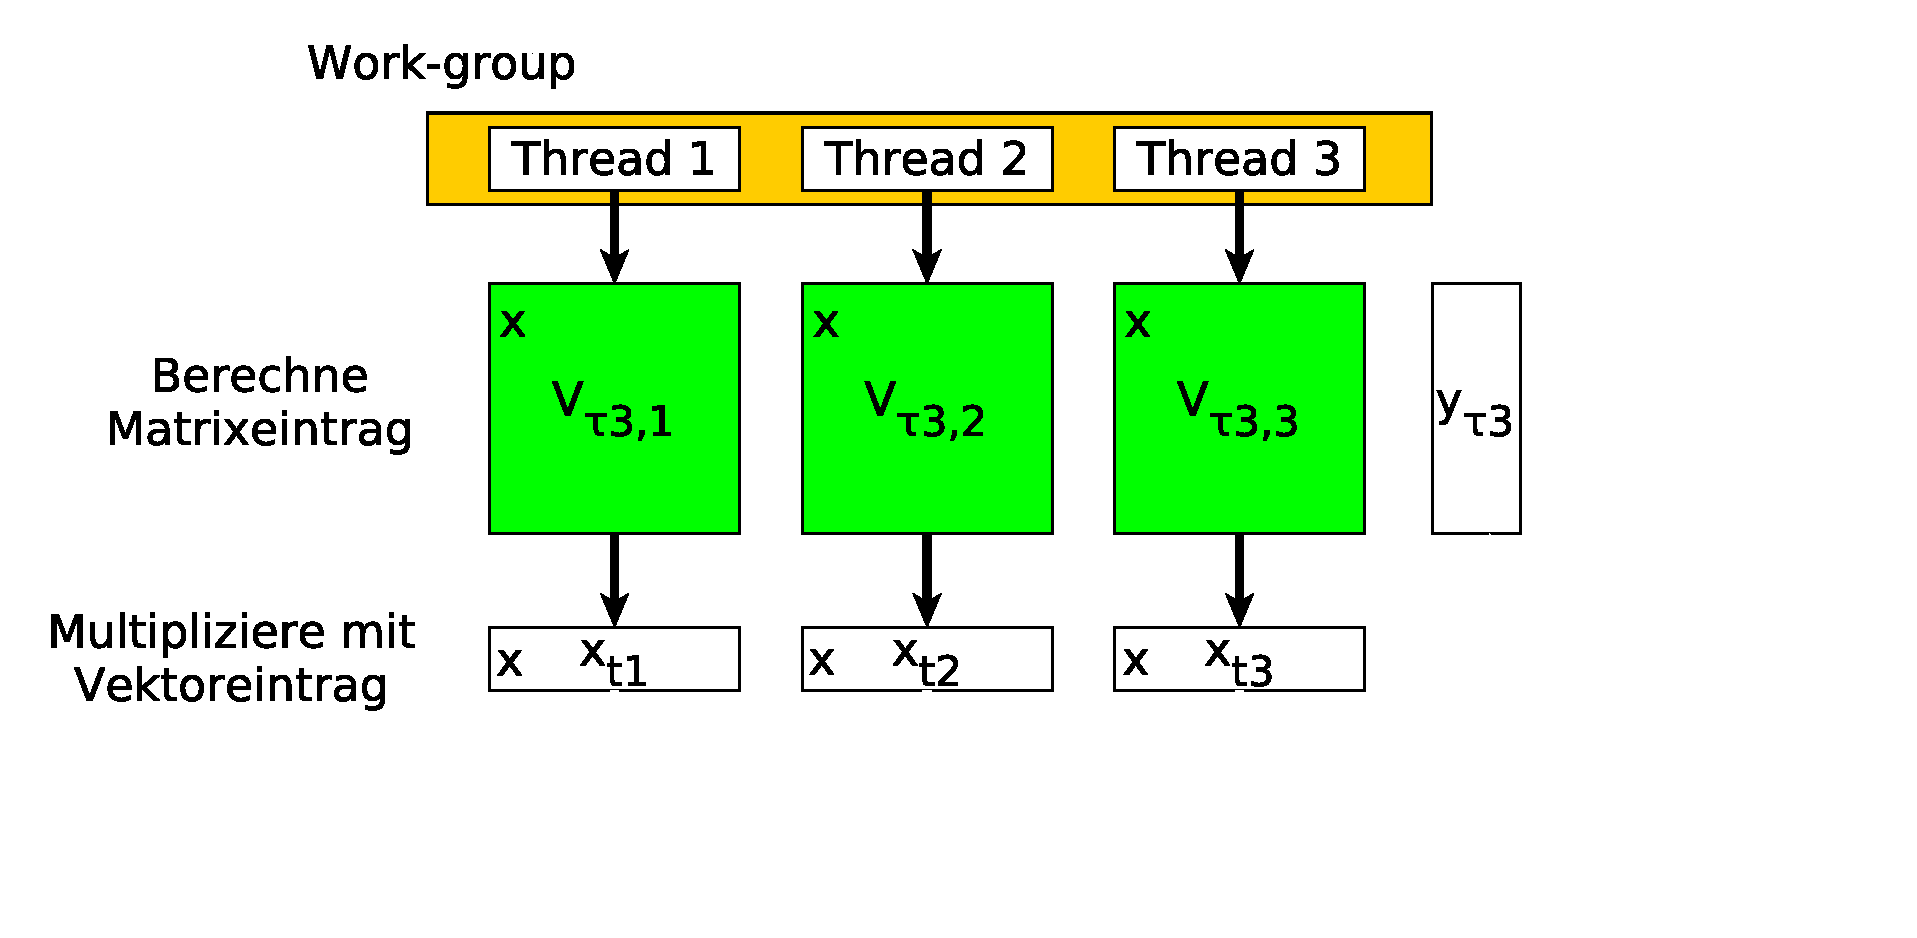
\includegraphics[width=\linewidth]{figures/fg-ff-multiply-vector.pdf}
        \caption{Multipliziere Matrix- mit Vektoreintrag.}
      \onslide<4>
        \centering
        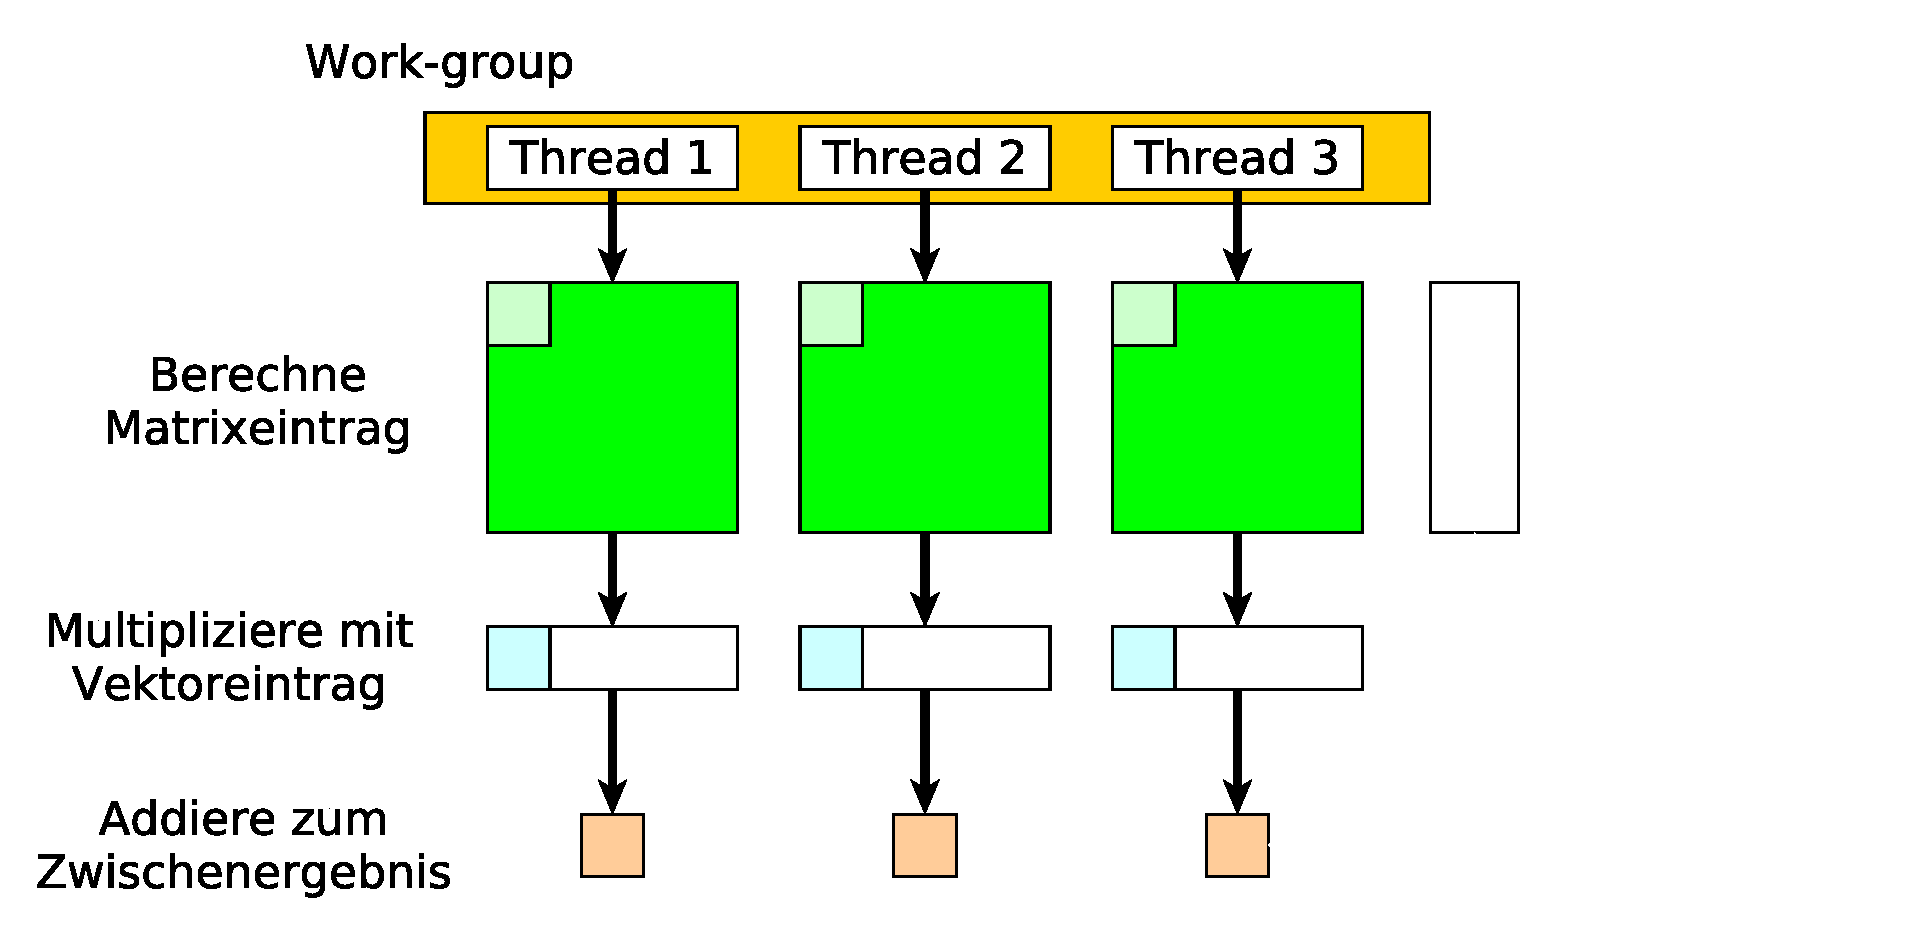
\includegraphics[width=\linewidth]{figures/fg-ff-add-interim-result.pdf}
        \caption{Addiere das Produkt zum Zwischenergebnis hinzu.}
      \onslide<5>
        \centering
        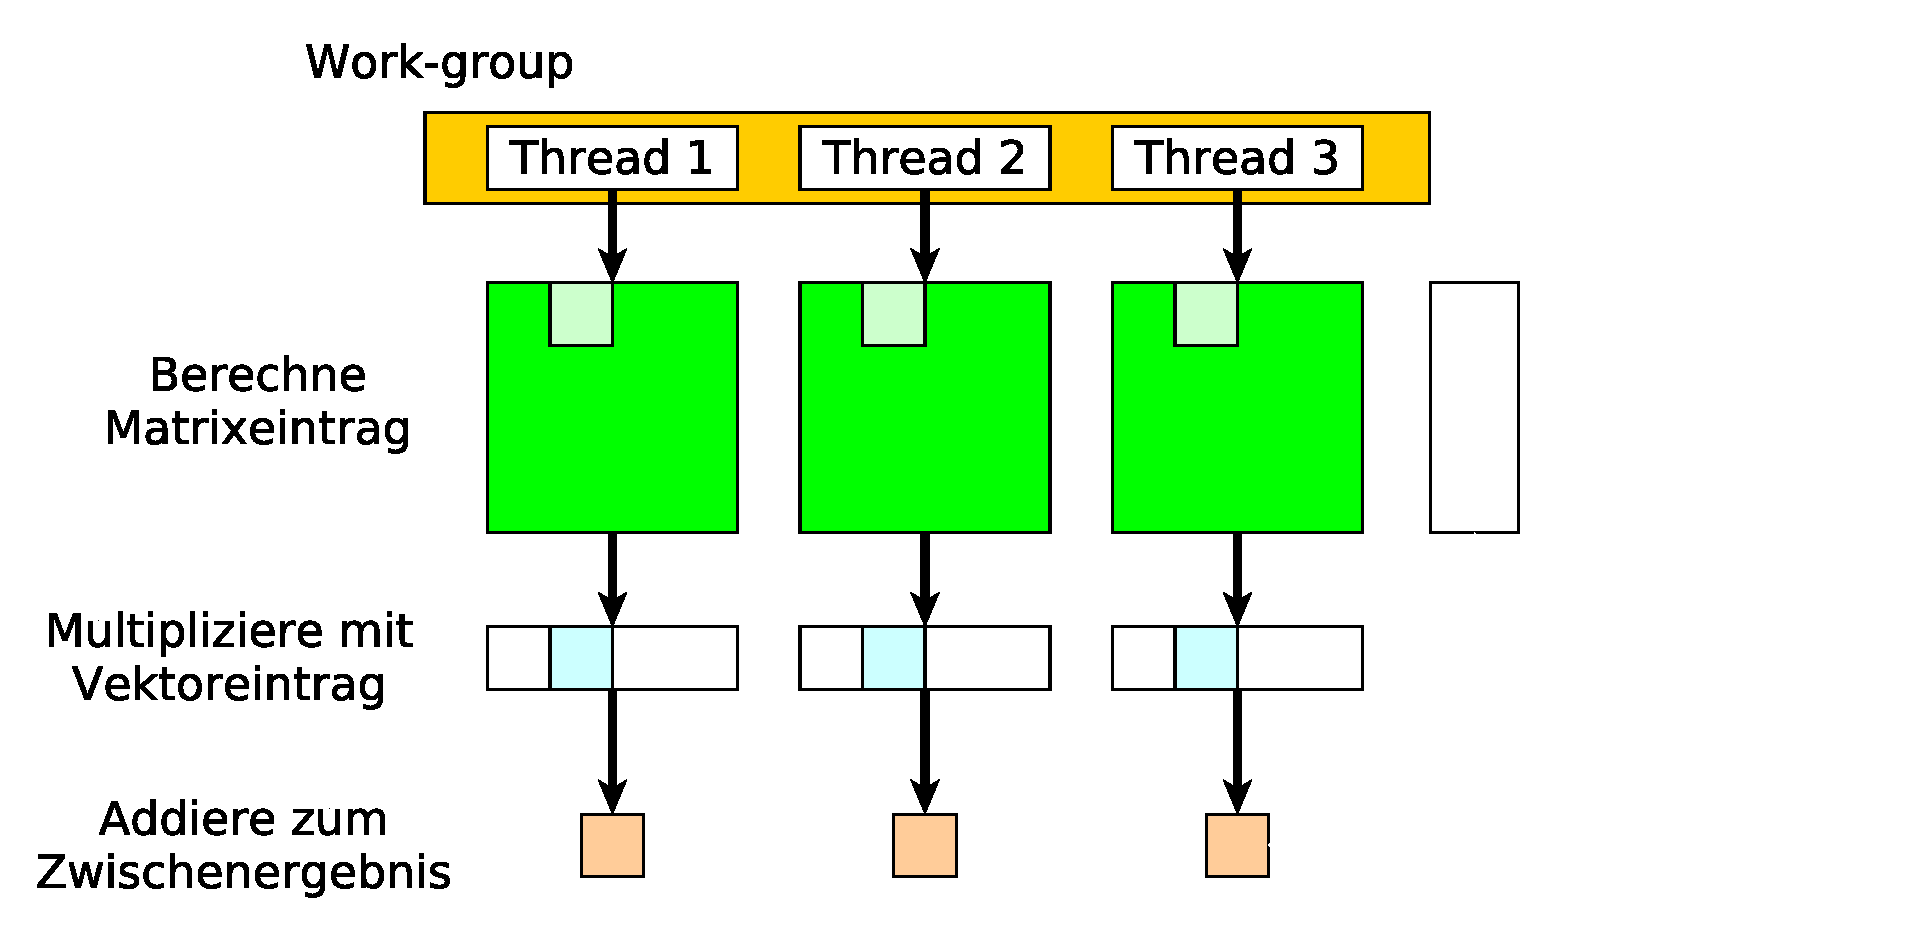
\includegraphics[width=\linewidth]{figures/fg-ff-next-column.pdf}
        \caption{Wiederhole die Prozedur f\"ur alle Eintr\"age einer Zeile.}
      \onslide<6>
        \centering
        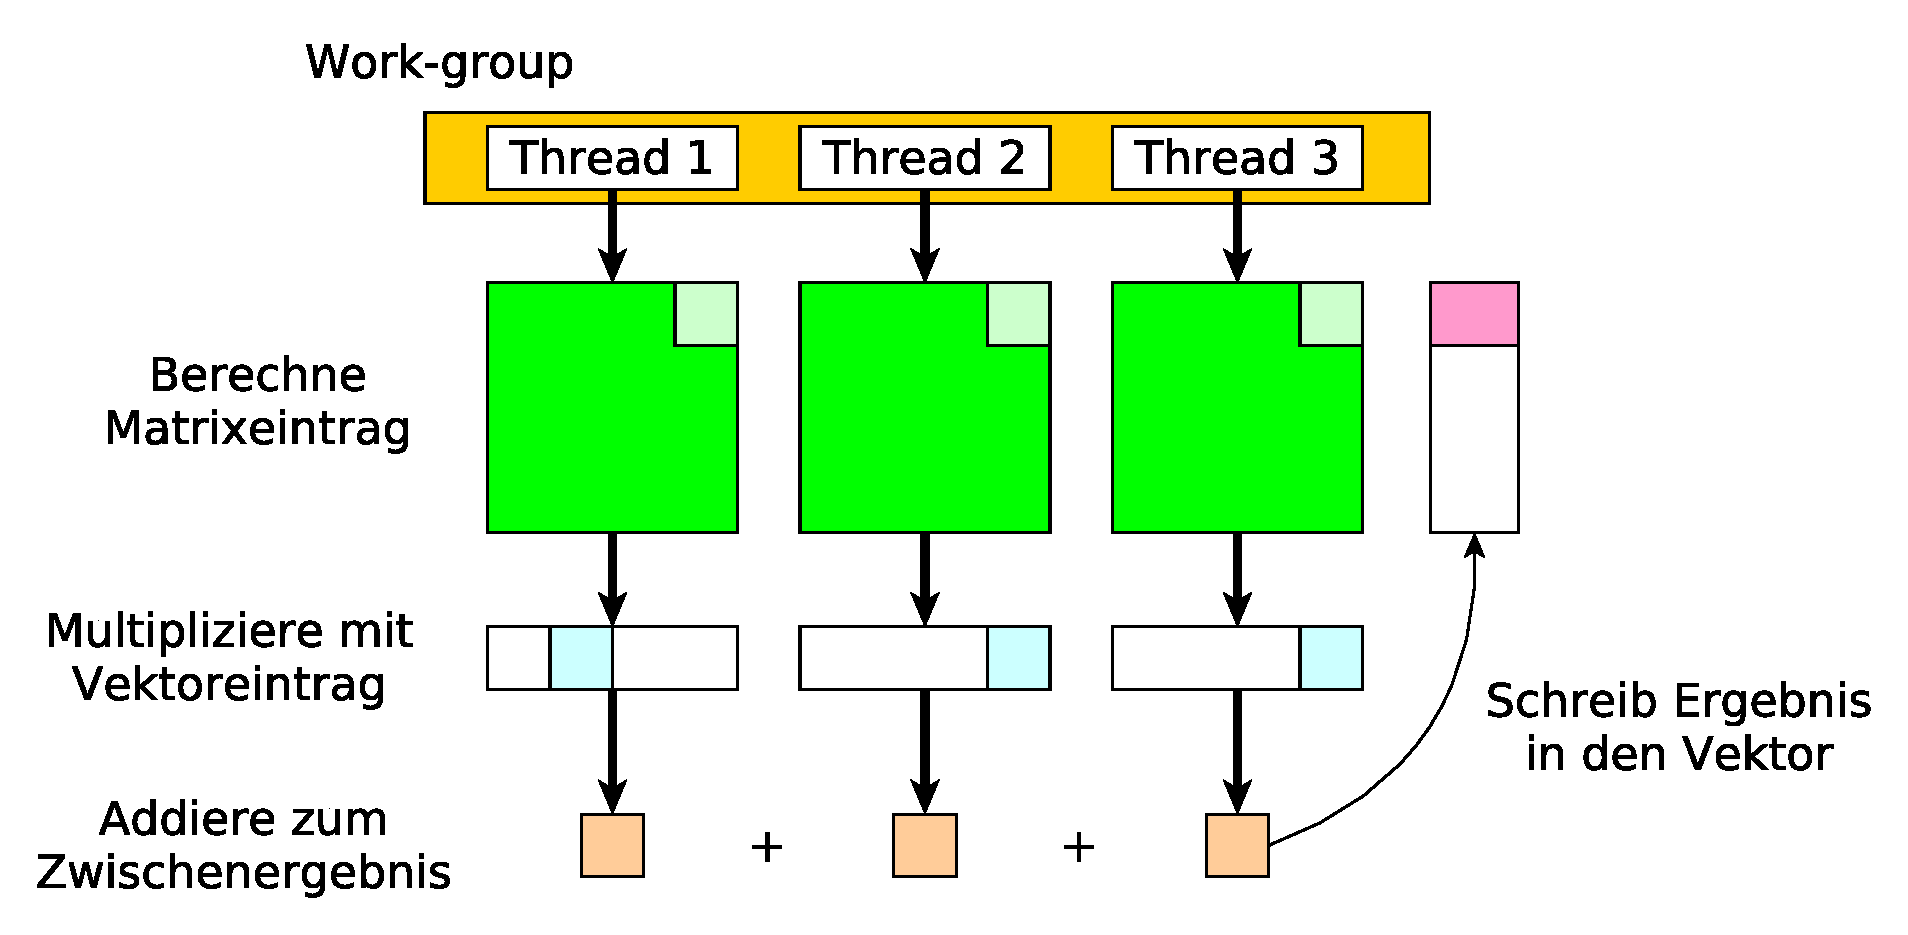
\includegraphics[width=\linewidth]{figures/fg-ff-write-result.pdf}
        \caption{Die Summe der Zwischenergebnisse ergibt den Eintrag im
                 Ausgabevektor.}
    \end{overprint}
  \end{figure}
\end{frame}

\begin{frame}{1. Phase (Fernfeld)}
  \begin{figure}
    \centering
    \includegraphics[width=\linewidth]{figures/fg-performance-ff.pdf}
    \caption{Rechenzeit der 1.~Phase auf verschiedenen GPUs.}
  \end{figure}
\end{frame}

\begin{frame}{1. Phase (Fernfeld)}
  \small
  \begin{table}
    \begin{tabular}{rrrrrr} \toprule
      \multirow{3}{*}{Dimension} & \multicolumn{5}{c}{Rechenzeit in ms\footnotemark[1]} \\ \cmidrule{2-6}
      & \multicolumn{2}{c}{CPUs\footnotemark[2]} & \multicolumn{3}{c}{GPUs} \\ 
      \cmidrule{2-6}
      & \begin{tabular}{@{}c@{}}Xeon \\ E5-4640\end{tabular}
      & \begin{tabular}{@{}c@{}}Core \\ i7-3820\end{tabular}
      & \begin{tabular}{@{}c@{}}Tesla \\ K20Xm\end{tabular}
      & \begin{tabular}{@{}c@{}}GeForce \\ GTX 680\end{tabular}
      & \begin{tabular}{@{}c@{}}GeForce \\ GTX 760\end{tabular} \\ \cmidrule{1-6}
       16\,384 &  16\,830 &  76\,423 &    367 &    430 &    469 \\
       32\,768 &  36\,960 & 167\,487 &    721 &    840 &    935 \\
       65\,536 &  74\,710 & 337\,433 & 1\,056 & 1\,182 & 1\,226 \\
      131\,072 & 154\,540 & 700\,738 & 2\,110 & 2\,387 &    --- \\
      \bottomrule
    \end{tabular}
  \end{table}
  \normalsize

  \footnotesize
  \footnotetext[1]{Gleikommazahlen einfacher Genauigkeit}
  \footnotetext[2]{Mit OpenMP parallelisiert und AVX beschleunigt.}
  \normalsize
\end{frame}

\begin{frame}{2.--3. Phase (Nahfeld)}
  \begin{itemize}
    \item Nahfeld besteht aus allen Integraltypen
    \item Approximation durch unterschiedliche Quadraturformeln
    \item Eckpunkte zweier Dreiecke müssen zueinander permutiert werden
  \end{itemize}
  
  \footnotesize
  \let\thefootnote\relax\footnote{S. A. Sauter und C. Lage.
  \href{https://link.springer.com/article/10.1007\%2Fs00211-015-0757-y}{
  ``On the efficient computation of singular and nearly singular surface 
  integrals arising in 3D-Galerkin BEM''}. In:   \textit{Zeitschrift f\"ur 
  angewandte Mathematik und Mechanik } 76 (1996), S. 273-275.}
  \addtocounter{footnote}{-1}\let\thefootnote\svthefootnote\relax
  \normalsize
\end{frame}

\begin{frame}{2.--3. Phase (Nahfeld)}
  \begin{overprint}
    \onslide<1>
      \begin{figure}
        \centering
        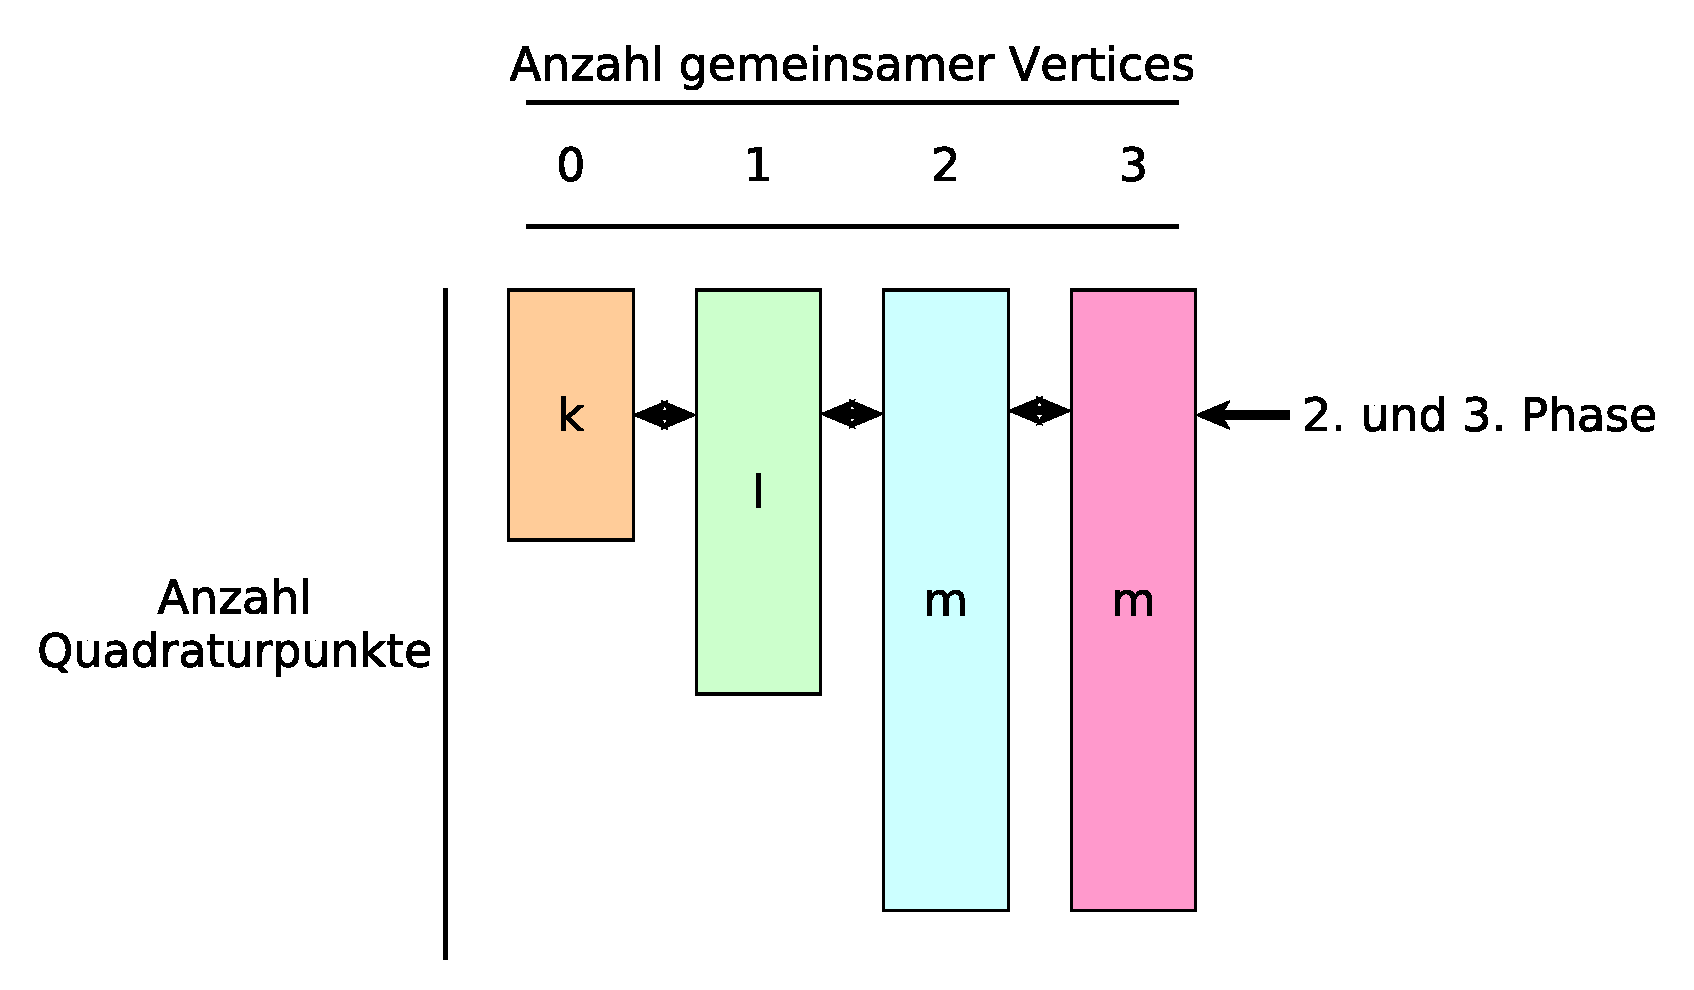
\includegraphics[width=.9\linewidth]{figures/fg-nf-quad-points.pdf}
      \end{figure}
    \onslide<2>
      \begin{figure}
        \centering
        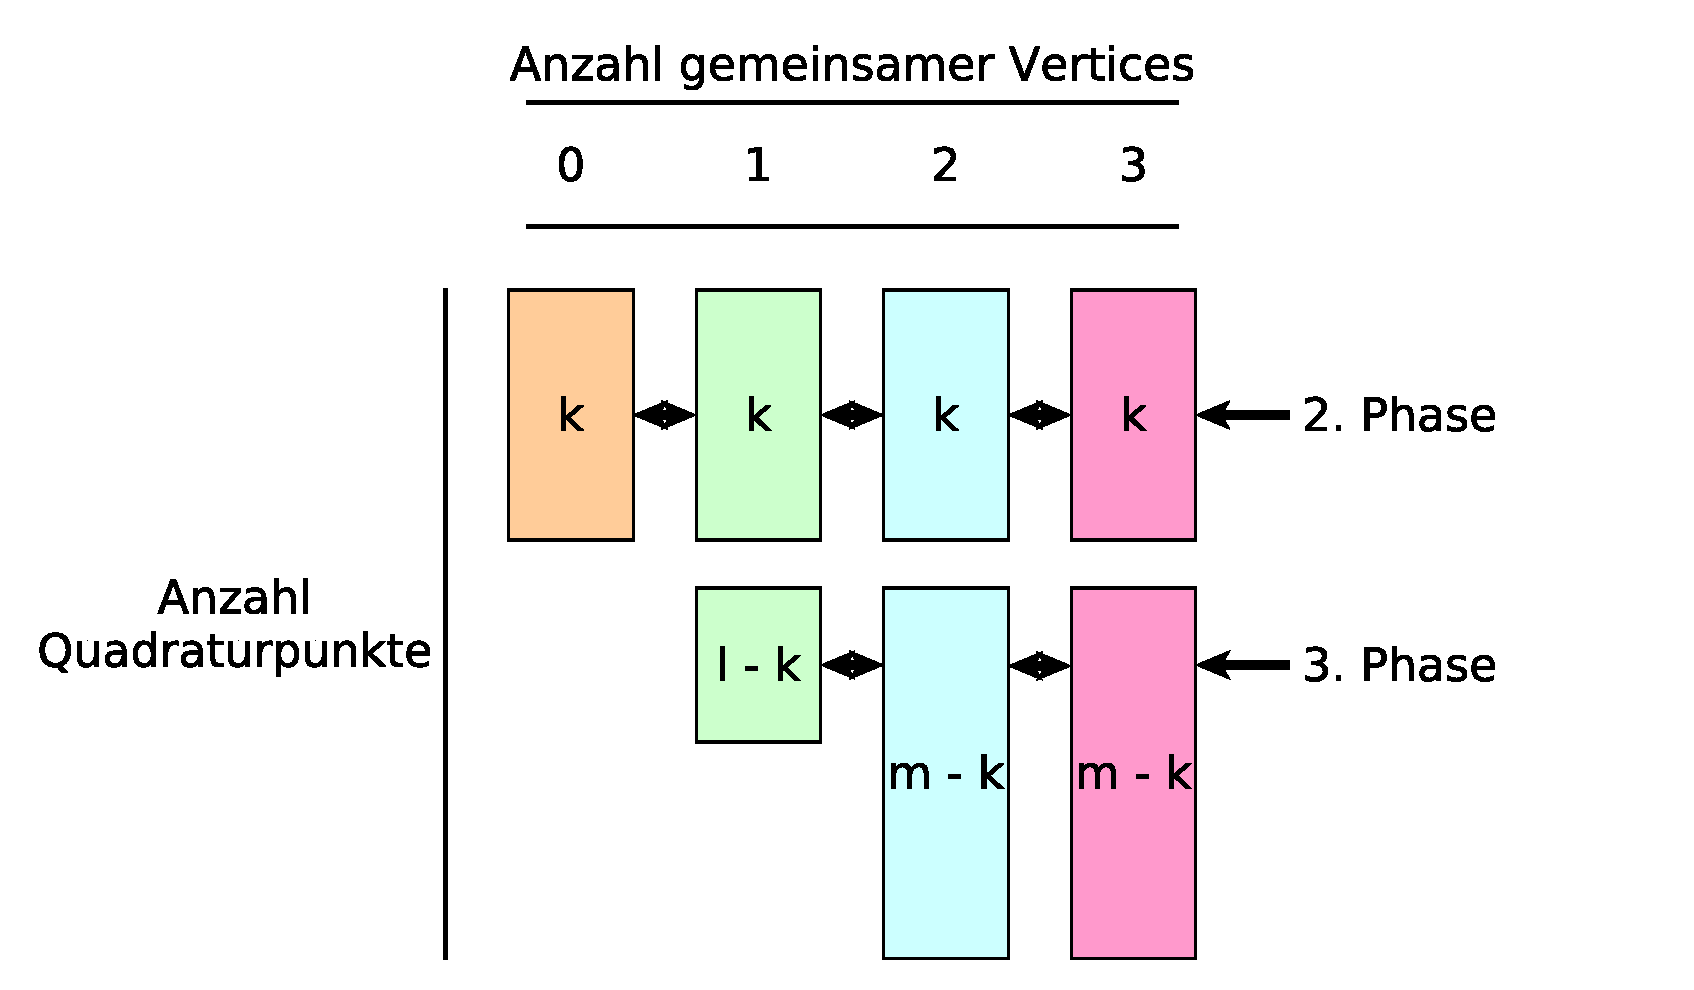
\includegraphics[width=.9\linewidth]{figures/fg-nf-quad-points-div.pdf}
      \end{figure}
  \end{overprint}

  \centerline{\( k, \ l, \ m \in \mathbb{N}, \ k < l < m\)}

  \footnotesize
  \let\thefootnote\relax\footnote{Steffen Börm u.\ a. \textit{H2Lib}.
  \url{http://www.h2lib.org/}.}
  \addtocounter{footnote}{-1}\let\thefootnote\svthefootnote\relax
  \normalsize
\end{frame}

\begin{frame}{2. Phase}
  \begin{itemize}
    \item \"Ahnlich wie in der 1. Phase, bis auf dass:
    \begin{itemize}
      \item f\"ur jeden Matrixeintrag entschieden werden muss, welche
            Quadraturformel zu wählen ist.
      \item f\"ur jeden Matrixeintrag die entsprechenden Dreiecksvertices
            zueinander permutiert werden müssen.
    \end{itemize}
  \end{itemize}
\end{frame}

\begin{frame}{2. Phase}
  \small
  \begin{table}
    \begin{tabular}{rrrrrr} \toprule
      \multirow{3}{*}{Dimension} & \multicolumn{5}{c}{Rechenzeit in ms} \\ \cmidrule{2-6}
      & \multicolumn{2}{c}{CPUs} & \multicolumn{3}{c}{GPUs} \\ \cmidrule{2-6}
      & \begin{tabular}{@{}c@{}}Xeon \\ E5-4640\end{tabular}
      & \begin{tabular}{@{}c@{}}Core \\ i7-3820\end{tabular}
      & \begin{tabular}{@{}c@{}}Tesla \\ K20Xm\end{tabular}
      & \begin{tabular}{@{}c@{}}GeForce \\ GTX 680\end{tabular}
      & \begin{tabular}{@{}c@{}}GeForce \\ GTX 760\end{tabular} \\ \cmidrule{1-6}
       16\,384 &    900 &  4\,547 &  72 &  64 &  75 \\
       32\,768 & 1\,780 &  9\,167 & 138 & 125 & 147 \\
       65\,536 & 3\,550 & 18\,162 & 273 & 246 & 291 \\
      131\,072 & 7\,070 & 36\,480 & 528 & 480 & --- \\
      \bottomrule
    \end{tabular}
  \end{table}
  \normalsize
\end{frame}

\begin{frame}{3. Phase}
  \begin{columns}
    \column{0.425\linewidth}
      \begin{algorithm}[H]
        \small{
          \( sum \gets 0 \) \;
          \For{\( q = 0 \to (nq - 1) \)}
          {
            \( sum \gets sum + w_{q} * kernel\relax(x_{q}, \ y_{q}) \) \;
          }
          \( result \gets result + sum \) \;
        }
      \end{algorithm}
    \column{0.6\linewidth}
      \begin{algorithm}[H]
        \small{
        \( lid \gets \) get\_local\_id\relax(0) \;
        \( lsize \gets \) get\_local\_size\relax(0) \;
        \( sum_{lid} \gets 0 \) \;
        \( q \gets 0 \) \;
        \While{\( q < nq \)}
        {
          \If{\( (q + lid) < nq \)}
          {
            \( sum_{lid} \gets sum_{lid} + w_{q + lid} *
               kernel\relax(x_{q + lid}, y_{q + lid}) \) \;
          }

          \( nq \gets nq + lsize \) \;
        }

        \( result \gets results + \sum\limits_{i = 0}^{lsize - 1} sum_{i} \) \;
        }
      \end{algorithm}
  \end{columns}
  \begin{center}
    Pseudocode zum sequentiellen (links) und Thread-Level-vektorisierten
    (rechts) Auswerten einer Quadratur.
  \end{center}
\end{frame}

\begin{frame}{3. Phase}
  \small
  \begin{table}[ht]\label{tab:fevalnfu}
    \begin{tabular}{rrrrrr} \toprule
      \multirow{3}{*}{Dimension} & \multicolumn{5}{c}{Rechenzeit in ms} \\
      \cmidrule{2-6}
      & \multicolumn{2}{c}{CPUs} & \multicolumn{3}{c}{GPUs} \\ \cmidrule{2-6}
      & \begin{tabular}{@{}c@{}}Xeon \\ E5-\relax4640\end{tabular}
      & \begin{tabular}{@{}c@{}}Core \\ i7-\relax3820\end{tabular}
      & \begin{tabular}{@{}c@{}}Tesla \\ K20Xm\end{tabular}
      & \begin{tabular}{@{}c@{}}GeForce \\ GTX 680\end{tabular}
      & \begin{tabular}{@{}c@{}}GeForce \\ GTX 760\end{tabular} \\ \cmidrule{1-6}
       16\,384 &    710 &  4\,005 &  95 & 122 & 109 \\
       32\,768 & 1\,420 &  8\,096 & 185 & 248 & 216 \\
       65\,536 & 2\,800 & 16\,019 & 359 & 463 & 433 \\
      131\,072 & 5\,680 & 32\,403 & 721 & 995 & --- \\
      \bottomrule
    \end{tabular}
  \end{table}
  \normalsize
\end{frame}


\begin{frame}{1.-3.Phase im Vergleich}
  \begin{figure}
    \centering
    \includegraphics[width=\linewidth]{figures/fg-performance-feval-1-3.pdf}
    \caption{Rechenzeit der einzelnen Phasen im Vergleich auf einer Tesla
             K20Xm.}
  \end{figure}
\end{frame}


\begin{frame}{Optimierung: Lokalit\"at von Speicher}
  \begin{algorithm}[H]
    \SetKwProg{Proc}{}{}{}
    \Proc{fastaddeval\_farfield}
    {
      \For{\( i = 0 \to (rows - 1) \)}
      {
        // Hole Informationen \"uber Zeile i \\
        \For{\( j = 0 \to (cols - 1) \)}
        {
          // Hole Informationen \"uber Spalte j \\

          \For{\( q = 0 \to (nq - 1) \)}
          {
            // F\"uhre Quadratur bzgl. i, j und q-ten Quadraturpunkt \\
            // und -gewicht durch.
          }
        }
      }      
    }
    \caption{Verschachtelte Schleifen in der 1. Phase. Eine tiefere
             Verschachtelungsebene bedeutet mehr Speicherzugriffe.}
  \end{algorithm}
\end{frame}

\begin{frame}{Optimierung: Lokalit\"at von Speicher}
  \begin{figure}
    \centering
    \includegraphics[width=\linewidth]{figures/fg-gpu_architecture.pdf}
    \caption{Erinnerung: (Speicher-)Architektur einer Grafikkarte.}
  \end{figure}
\end{frame}

\begin{frame}{Optimierung: Lokalität von Speicher}
  \small
  \begin{table}
    \begin{tabular}{rrr} \toprule
      \multirow{3}{*}{Dimension} & \multicolumn{2}{c}{Rechenzeit in ms} \\ \cmidrule{2-3}
      & \multicolumn{2}{c}{Lokalität der Quadraturpunkte} \\ \cmidrule{2-3}
      & Globaler Speicher & Lokaler Speicher \\ \cmidrule{1-3}
       16\,384 &    367 &    305  \\ %324 bytes
       32\,768 &    721 &    614  \\
       65\,536 & 1\,056 &    805  \\
      131\,072 & 2\,110 & 1\,665 \\
      \bottomrule
    \end{tabular}
    \caption{Performanzvergleiche der Verfügbarkeit von Quadraturpunkten
             in unterschiedlichen Speicherbereichen auf einer Tesla K20Xm.}
  \end{table}
  \normalsize
\end{frame}

\begin{frame}{Optimierung: Vektorisierung auf Instruktionsebene}
  \begin{itemize}
    \item z.\,B. float2, float4, float8, float16 in OpenCL
    \item Abstrahieren die Vektorregister der unterliegenden Architektur
    \item SSE/AVX auf CPUs (falls vorhanden)
    \item NVIDIAs Skalarprozessoren besizten keine Vektoreinheiten
    \begin{itemize}
      \item Vektorisierte Speicherzugriffe können jedoch zusammengefasst
            werden.
      \item Vektorisierte Rechenoperationen werden durch skalare simuliert
      \item Höhere Anzahl an Register werden benötigt
    \end{itemize}
  \end{itemize}
\end{frame}

\begin{frame}{Optimierung: Vektorisierung auf Instruktionsebene}
  \begin{table}[ht]\label{tab:vec}
    \begin{tabular}{rrr} \toprule
      \multirow{3}{*}{Dimension} & \multicolumn{2}{c}{Rechenzeit in ms} \\ 
      \cmidrule{2-3}
      & \multicolumn{2}{c}{Vektorbreite} \\ \cmidrule{2-3}
      & 1 & 4 \\ \midrule
       16\,384 &    305 &    286 \\
       32\,768 &    614 &    581 \\
       65\,536 &    805 &    763 \\
      131\,072 & 1\,665 & 1\,562 \\
      \bottomrule
    \end{tabular}
    \caption{Vergleich der Rechenzeit unterschiedlicher Vektorbreiten, 
             verwendet zur vektorisierten Berechnung der Quadratur.}
  \end{table}
\end{frame}

\section{Zusammenfassung \& Ausblick}

\begin{frame}{Zusammenfassung}
  \begin{table}[ht]\label{tab:mvm}
    \resizebox{\textwidth}{!}
    {
      \begin{tabular}{rrrrrrrr} \toprule
        \multirow{4}{*}{Dimension} & \multicolumn{7}{c}{Rechenzeit in ms} \\
        \cmidrule{2-8}
        & \multirow{3}{*}{\( \mathcal{H}^2 \)-MVM}
        & \multicolumn{6}{c}{Ordnung} \\ \cmidrule{3-8}
        & & \multicolumn{2}{c}{2} & \multicolumn{2}{c}{3} & \multicolumn{2}{c}{4}
        \\ \cmidrule{3-8}
        & 
        & \begin{tabular}{@{}c@{}}
            \( \mathcal{H}^2 \)-MVM \\
            (CPU)
          \end{tabular}
        & \begin{tabular}{@{}c@{}}
            \( \mathcal{H}^2 \)-MVM \\
            (GPU)
          \end{tabular}
        & \begin{tabular}{@{}c@{}}
            \( \mathcal{H}^2 \)-MVM \\
            (CPU)
          \end{tabular}
        & \begin{tabular}{@{}c@{}}
            \( \mathcal{H}^2 \)-MVM \\
            (GPU)
          \end{tabular}
        & \begin{tabular}{@{}c@{}}
            \( \mathcal{H}^2 \)-MVM \\
            (CPU)
          \end{tabular}
        & \begin{tabular}{@{}c@{}}
            \( \mathcal{H}^2 \)-MVM \\
            (GPU)
          \end{tabular} \\ \midrule
         16\,384 &    140 &  6\,980 &    500 &  19\,770 &    950 &  50\,730 &
          2\,350 \\
         32\,768 &    300 & 14\,640 & 1\,000 &  43\,600 & 1\,820 & 106\,770 &
          4\,530 \\
         65\,536 &    660 & 29\,440 & 1\,490 &  94\,740 & 2\,940 & 220\,670 &
          8\,280 \\
        131\,072 & 1\,190 & 60\,920 & 3\,030 & 194\,980 & 5\,840 & 452\,060 & 
         16\,320 \\
        \bottomrule
      \end{tabular}
    }
  \end{table}
  \begin{itemize}
    \item Wir können den Speicherbedarf einer \(\mathcal{H}^2\)-Matrix um
          75 bis 90\,\% reduzieren
    \item Die benötigte Rechenzeit kann auf GPUs um einen Faktor 20 bis 50
          verglichen mit einer CPU-Implementierung reduziert werden
    \item Rechenaufwand jedoch höher als bei einer reinen
          Matrix-Vektor-Multiplikation (und nimmt zusätzlich mit höherer
          Quadraturordnung zu)
  \end{itemize}
\end{frame}

\begin{frame}{Zusammenfassung}
  \small
  \begin{table}
    \begin{tabular}{rrr} \toprule
                & \multicolumn{2}{c}{Performanz in ms} \\ \cmidrule{2-3}
      Dimension & \(\mathcal{H}^2\)-Matrix & Blockmatrizen \\ \midrule
          16\,384 &                     131\,620 &   63\,310 \\
          32\,768 &                     267\,940 &  109\,092 \\
          65\,536 &                     530\,570 &  271\,120 \\
         131\,072 &                  1\,073\,480 &  559\,450 \\ \bottomrule
      \end{tabular}
    \end{table}
  \normalsize
  \begin{itemize}
    \item Setup-Zeit lässt sich um die Hälfte reduzieren
  \end{itemize}
\end{frame}

\begin{frame}{Ausblick}
  \begin{itemize}
    \item Parallelisierung des hostseitigen Codes?
    \item Multi-GPU\@?
    \item Auslagern der Vorwärts- und Rückwärtstransformation auf GPUs?
  \end{itemize}
\end{frame}

\begin{frame}[allowframebreaks]{Literatur}

  \printbibliography{}
  \nocite{*}

\end{frame}

\begin{frame}
  \centerline{\Huge Vielen Dank! Fragen?}
\end{frame}
\end{document}
